\section{一元函数的可测性和积分}
\label{sec:analysis-measurability-integration}
\label{sec:analysis-integration-average}
\label{sec:analysis-classical-integration}

上一节已经回答怎样测量集合的大小，现在进一步问：函数在不同位置取不同值时，怎样结合这些值与所在范围的大小，得到一个累计量？
例如，密度恒为$c$的一段区间长为$\ell$，总质量就是$c\ell$；密度随位置变化时，需要把这种计算推广到一般函数。
本节的自变量始终是一维实变量，有限区间先取$a<b$。

先沿输入区间分段取样，建立黎曼积分，检验分割越来越细时取样结果能否稳定。
狄利克雷函数将说明，有些函数的非零取值虽然只落在零测集上，每个短区间的取样却仍可能给出完全不同的累计。
为处理这种情形，我们利用第~\ref{sec:comb-set-measurement}节的可测集合与测度，改按函数取值划分输入，
先定义哪些函数能够这样分层，再以简单函数的有限累计构造勒贝格积分。

这条路线中的条件各有作用：可测集合提供允许测量的范围，测度给这些范围赋值，可测函数保证取值分层落在该范围内，
可积条件再保证总累计有限。它们不能互相替代。
在两种积分的定义和关系明确后，我们再研究累计函数与求导的联系、有限运算、函数列与函数项级数的极限交换以及反常积分；每一步都说明所用的是哪种积分及相应条件。

\subsection{黎曼定积分}
\label{sec:analysis-integral-definitions}
\label{sec:analysis-riemann-integral}

先保留区间长度作为权重，研究把输入切成小段后能否得到与取样无关的总量。这里使用有限区间分割，尚不需要一般可测集合的积分。


\subsubsection{积分的定义}

从常数密度乘长度的计算出发，先构造有限近似，再用所有足够细的近似是否稳定来定义积分。误差控制必须同时覆盖分割与取样两种选择。


\paragraph{区间分割}
要累计$f$在$[a,b]$上的取值，先把区间分成有限段。取
\[
 P:\quad a=x_0<x_1<\cdots<x_n=b,
\]
称$P$为一个分割，记$\Delta x_i=x_i-x_{i-1}$，$\lVert P\rVert=\max_i\Delta x_i$。分割的细度$\lVert P\rVert$衡量最长小段的长度；让它趋零，要求每段都变短，而不只是增加分割点的数量。

\paragraph{黎曼和}
在每个小区间中取样点$\xi_i\in[x_{i-1},x_i]$，用常数$f(\xi_i)$代表该段的函数值，得到
\[
 S(f,P,\xi)=\sum_{i=1}^n f(\xi_i)\Delta x_i.
\]
这称为\term{黎曼和}（Riemann sum）。若$f\geq0$，每项是一个矩形的面积；有负值时，位于横轴下方的矩形按负号计入，所以求和表示带符号的累计。

\paragraph{黎曼积分}
区间分得越来越细时，不同取样方式所得的黎曼和仍可能不同。只有当这些取样结果都趋向同一个有限值时，才能把这个值作为函数在区间上的累计量。

\begin{definition}[黎曼积分]
\label{def:analysis-riemann-integral}
设$f:[a,b]\to\mathbb R$有界。若存在实数$A$，使对每个$\varepsilon>0$都存在$\delta>0$，当$\lVert P\rVert<\delta$时，不论怎样选取样点都有
\[
 |S(f,P,\xi)-A|<\varepsilon,
\]
则称$f$在$[a,b]$上\term{黎曼可积}（Riemann integrable），并称$A$为其\term{黎曼积分}（Riemann integral），记为$\int_a^bf(x)\,\mathrm dx$。
\end{definition}
积分值必须独立于足够细的分割及其中的取样点。例如$f(x)=c$时，每个黎曼和都等于$c(b-a)$，所以积分就是$c(b-a)$。对更一般的函数，下一小节将用上下和判断这种共同极限是否存在。

\paragraph{定积分与积分变量}
固定被积函数和积分范围后，$\int_a^bf(x)\,\mathrm dx$是一个数，称为定积分；$a,b$分别为下限和上限，$x$为积分变量。积分变量只在积分式内部使用，换成$t$不改变结果：$\int_a^bf(x)\,\mathrm dx=\int_a^bf(t)\,\mathrm dt$。采用有向端点约定$\int_b^af=-\int_a^bf$及$\int_a^af=0$。以后定义的勒贝格积分也有固定范围的定积分，但采用的可积条件不同。

\subsubsection{可积性的要求}
\label{sec:analysis-integrability-requirements}

有界性保证每个有限黎曼和有意义，却不能保证所有细分与取样得到共同极限。上下和将不同取样的可能结果夹住，使可积性成为可以验证的误差条件。

\paragraph{上和与下和}
取样点可能选到小段中不同的函数值。为了同时控制全部选择，设$f$在$[a,b]$上有界，对分割$P$定义
\begin{equation}
 \begin{aligned}
 m_i&=\inf_{[x_{i-1},x_i]}f,\qquad M_i=\sup_{[x_{i-1},x_i]}f,\\
 L(f,P)&=\sum_i m_i\Delta x_i,\qquad
 U(f,P)=\sum_i M_i\Delta x_i.
 \end{aligned}
\label{eq:analysis-riemann-upper-lower-sums}
\end{equation}
$L$称为下和，$U$称为上和，任意黎曼和都夹在它们之间。这里使用上确界和下确界，是因为有界函数在小段上未必达到最大、最小值。

\paragraph{Darboux判据}
增加分割点不会减小下和，也不会增大上和。任意两个分割有公共加细，因而任意下和都不超过任意上和。定义下积分$\sup_PL(f,P)$、上积分$\inf_PU(f,P)$；有界函数黎曼可积，当且仅当两者相等，等价地，对每个$\varepsilon>0$存在分割$P$满足
\[
 U(f,P)-L(f,P)<\varepsilon.
\]
这称为Darboux判据。上下积分相等时，分别取接近它们的分割并公共加细，即得上述小差；反之，小差直接夹住两种积分的差。

还须把它与任意细分割的黎曼和联系起来。固定一个上下和差很小的分割$P_0$，设它有$k$个内分割点，且$|f|\leq M$。对另一个分割$Q$，只有跨过这些分割点的至多$k$个小段无法直接沿用$P_0$的上下界，其总长度至多为$k\lVert Q\rVert$；对这些段，函数振幅至多$2M$。因此
\[
 U(f,Q)-L(f,Q)\leq U(f,P_0)-L(f,P_0)+2Mk\lVert Q\rVert.
\]
令$\lVert Q\rVert$足够小，就能把所有取样黎曼和夹到共同的上下积分附近。反过来，若所有细分割的黎曼和都接近同一个值，在每个小段上分别选接近上确界、下确界的取样点，便得到上下和差任意小。这证明了两种定义等价。

\paragraph{连续函数的可积性}
先把上下和误差条件用于已经研究过的连续函数，检验它是否给出所期待的累计。
若$f$在$[a,b]$上连续，闭区间性质先保证有界和一致连续。给定$\varepsilon>0$，取$\delta$使输入距离小于$\delta$时，输出距离小于$\varepsilon/[2(b-a)]$。选细度小于$\delta$的分割，则
\[
 U(f,P)-L(f,P)=\sum_i(M_i-m_i)\Delta x_i\leq\varepsilon/2<\varepsilon.
\]
所以闭区间上的连续函数黎曼可积。一致连续性在这里提供了对全部小区间都适用的分割尺度。

\paragraph{有限间断点函数的可积性}
少数位置上的不连续是否必然破坏累计，要看能否用很短的区间隔离这些位置，再控制其余范围。
连续性是可积的充分条件，未必必要。若有界函数只在有限个点不连续，先用总长度任意小的区间包住它们，这些段的上下和差不超过函数总振幅乘总长度；剩余部分由有限个闭区间组成，函数在其上连续，可用一致连续性控制上下和差。因此它也黎曼可积。有限处跳跃而其余位置连续的有界函数，以及连续函数在有限个点作有限改值所得的函数，都属于这种情形。

\paragraph{区间分拆与基本估计}
微积分基本定理要比较相邻端点的累计，先从定义建立所需的两项性质。若$f$在$[a,b]$上黎曼可积，则它在每个子区间上也黎曼可积：把子区间端点加入分割，下、上和的非负差在该子区间上不超过全区间的差。对$a\leq c\leq b$分别取两侧黎曼和，再合并分割，求和恒等式给出
\[
 \int_a^bf=\int_a^cf+\int_c^bf.
\]
同样，取样和的加减、数乘直接给出黎曼积分的线性。后面的运算法则统一采用勒贝格积分，其线性将从简单函数构造另行建立。若$m\leq f\leq M$，每个取样和都夹在$m(b-a)$与$M(b-a)$之间，所以积分也被这两个量夹住。特别地，$|f|\leq M$时有$|\int_a^bf|\leq M(b-a)$；区间方向反转时用绝对长度估计。这些结论只用有限和与其极限，不依赖基本定理。


图~\ref{fig:analysis-process-riemann-upper-lower}显示分割加细怎样缩小上和与下和之间的差距。
\begin{figure*}[!htbp]
 \centering
 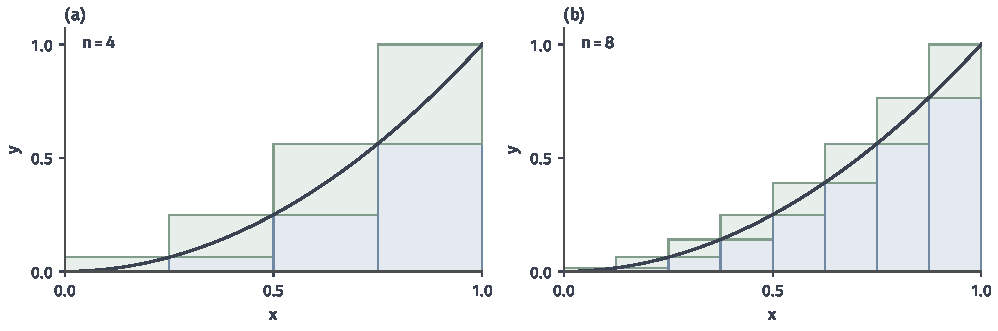
\includegraphics[width=169.0mm]{figures/01-mathematical-preliminaries-upper/01-mathematical-language-combinatorics-analysis-optimization/matplotlib/chapter3-concept-processes/riemann-upper-lower.pdf}
 \caption{对$[0,1]$上的$f(x)=x^2$，分别等分为4段、8段。蓝色矩形累计下和，补上绿色部分得到上和，黑线为函数图像。两种颜色之间的面积差是$U_n-L_n=1/n$，从$1/4$降到$1/8$；Darboux判据要求这种差能任意小，而不只是选定一张图时较小。}
 \label{fig:analysis-process-riemann-upper-lower}
\end{figure*}

\subsubsection{黎曼积分的局限}

连续函数以及只有有限个间断点的有界函数都已证明黎曼可积，但这不能说明任意有界函数都能通过细分区间累计。下面用同一个零测点集构造反例，并说明这与积分在函数极限下的稳定性有什么关系。


\paragraph{狄利克雷函数}
前面的可积条件要求各段振幅乘长度后的总误差趋零。现在考察一个有界函数，说明仅靠继续缩短输入区间，可能始终无法减小这种误差。
令$Q_0=\mathbb Q\cap[0,1]$，$d(x)=\mathbb I_{Q_0}(x)$，称为狄利克雷函数。
每个非退化小区间都含有有理数和无理数，所以任意分割的每段都有$m_i=0$、$M_i=1$，从而
\[
 L(d,P)=0,\qquad U(d,P)=1.
\]
即使分割任意细，全部选有理取样点会得到黎曼和$1$，全部选无理取样点会得到$0$。
这不是取样还不够密，而是“所有细分割与所有取样都给出共同极限”的要求在这里不成立，因此$d$不黎曼可积。

上一节已经证明$m(Q_0)=0$、$m([0,1]\setminus Q_0)=1$。若按这两个取值集合累计，取值$1$只对应零测范围，取值$0$对应其余范围，所需的有限计算便是
\[
 1\cdot m(Q_0)+0\cdot m([0,1]\setminus Q_0)=0.
\]
这提示我们，扩大积分范围可以改变分组依据：不再只用相邻输入的小区间代表函数，而允许把具有同一取值的输入归为一组。

黎曼方法在极限过程中还有同样的范围障碍。列举$Q_0=\{q_1,q_2,\ldots\}$，令$d_n=\mathbb I_{\{q_1,\ldots,q_n\}}$。
每个$d_n$只在有限点非零，黎曼可积且积分为$0$；它们却逐点递增到不黎曼可积的$d$。
所以各步都能积分，并不保证极限仍能用同一定义积分。后面将看到，新的分层累计既能处理$d$，也能在非负单调逼近下保留积分极限。

这并不否定黎曼积分在连续函数等情形中的作用。新的构造还必须证明，在原来黎曼可积的范围内，它与已有积分相等。

\subsection{勒贝格定积分}
\label{sec:analysis-lebesgue-definite-integral}

狄利克雷函数已经给出两个可测取值集合，因而能按“函数值乘相应集合的测度”计算。
一般函数可能取无限多个值，需要先把取值范围分成有限档，再逐步缩小档宽并提高截断高度。
每一档对应的输入集合可能散布在许多位置，不再要求是一个区间。

这时前一节的测量结构分别承担明确任务：$\sigma$代数保证各档集合及其可数运算仍在允许范围内，测度为每档赋予大小。
还缺的条件在函数一侧：由它划出的各档是否可测？这就是先引入可测函数的原因。
保证分层有意义之后，再定义有限档的简单函数积分、非负函数的积分，最后检查有符号累计是否有限。

\subsubsection{可测函数}
\label{sec:analysis-measurable-functions}

按取值分层之前，必须先给函数一个资格条件：这些层在输入端是否属于已选的可测范围。这个条件只负责能否测量，不负责总量是否有限。


\paragraph{可测函数的定义}
可测集是输入范围中的集合，可测函数则要保证：指定输出的一段取值范围后，落入这段范围的输入仍组成可测集。
例如要计算取值大于$c$的输入占多大测度，必须先有$\{x:f(x)>c\}\in\mathcal A$，才能使用$\mu$对它赋值。

一般地，输出范围取Borel集$B\subseteq\mathbb R$，分层累计的对象关系是
\[
 B\longmapsto f^{-1}(B)=\{x\in X:f(x)\in B\}
 \longmapsto\mu(f^{-1}(B)).
\]
这里对输入集合使用$\mu$，没有把函数值本身当成集合的测度。
下面用所有Borel原像可测的要求规定函数的可测性。
\begin{definition}[可测函数]
\label{def:analysis-measurable-function}
设$X\subseteq\mathbb R$，$(X,\mathcal A,\mu)$为测度空间。函数$f:X\to\mathbb R$称为\term{可测函数}（measurable function），若对每个Borel集$B\subseteq\mathbb R$，原像$f^{-1}(B)$都属于$\mathcal A$。等价地，只需对每个$a\in\mathbb R$有$\{x\in X:f(x)>a\}\in\mathcal A$。扩展实轴$[-\infty,+\infty]$的Borel结构由射线$(a,+\infty]$（$a\in\mathbb R$）生成，扩展实值函数按此结构作同样定义。
\end{definition}
阈值条件之所以足够，是因为射线$(a,\infty)$生成实轴的Borel $\sigma$代数，且原像保持补集与可数并。
具体地，所有原像属于$\mathcal A$的输出集合本身构成一个$\sigma$代数；若它包含全部射线，就包含这些射线生成的全部Borel集。
因此，既可以逐个检验阈值集合，也可以直接使用Borel原像条件。

例如一档取值$[u,v)$对应$\{u\leq f<v\}$，它是Borel集$[u,v)$的原像，因而可测。
对于狄利克雷函数，各档的原像只可能是$\varnothing,Q_0,[0,1]\setminus Q_0,[0,1]$，都勒贝格可测。
所以它虽不满足黎曼可积要求，却已经具备新构造所需的分层资格；这还没有替任意函数保证积分有限。
反过来，若$A\subseteq X$不属于$\mathcal A$，示性函数$\mathbb I_A$就不可测，因为$\{\mathbb I_A>1/2\}=A$。
此时连非零取值落在哪个可测范围内都无法满足要求，不能直接套用“取值乘测度”的规则。

可测性还依赖指定的$\sigma$-代数。例如$X=\{0,1\}$上仅取$\mathcal A=\{\varnothing,X\}$，函数$f(0)=0,f(1)=1$不可测，因为$\{f>1/2\}=\{1\}\notin\mathcal A$；若改取幂集$\mathcal P(X)$，同一函数就可测。

\paragraph{连续函数与可测函数}
新的函数范围应包含原来熟悉的连续函数，同时容纳促使我们改变积分构造的狄利克雷函数。
在实轴Borel结构下，连续函数可测，因为开集的原像是开集。若定义域使用包含Borel集的勒贝格可测结构，结论仍成立。反之，可测函数不必连续：狄利克雷函数的两个取值集合都勒贝格可测，所以它可测，却在每一点间断。

\paragraph{可测函数的运算}
分层累计还要用于函数的加减、相乘和复合，因此应先保证这些运算不会把函数带出可测范围。
实值可测函数的和、积、绝对值、最大值与最小值仍可测。以和为例，
\[
 \{f+g>a\}=\bigcup_{q\in\mathbb Q}\bigl(\{f>q\}\cap\{g>a-q\}\bigr),
\]
右侧为可数个可测集合的并。连续实函数与可测函数复合仍可测，因而平方和绝对值可测；再由$fg=((f+g)^2-(f-g)^2)/4$得到乘积可测。最大、最小可由绝对值表达。商在分母不为零的可测集合上可测；若要扩展到全域，需另行指定零点处的可测取值。

对两个一般可测映射，复合还须核对中间可测结构：若$f:(X,\mathcal A)\to(Y,\mathcal B)$和$g:(Y,\mathcal B)\to(Z,\mathcal C)$可测，则$(g\circ f)^{-1}(C)=f^{-1}(g^{-1}(C))\in\mathcal A$。仅说两个实函数各自勒贝格可测，不能跳过中间结构就认定任意复合也可测。扩展实值运算还要排除$\infty-\infty$等未定义形式。

\subsubsection{积分的定义}

测度已经能计算可测集合的大小，现在先把它接到有限取值函数上，再借助下方逼近得到一般非负函数的累计。最后通过正负分解处理带符号取值。


\paragraph{简单函数}
先处理只取有限多个值的可测函数：若它在可测集$E_j$上恒为$a_j$，该组的贡献就应为$a_j\mu(E_j)$。
把各组取为两两不交后，每个输入只计一次，这正是前一节测度有限可加性所支持的累计方式。
下面先对非负取值定义积分，有负取值时稍后再拆成正负两部分。
\begin{definition}[简单函数及其积分]
\label{def:analysis-simple-function-integral}
只取有限个实数值的可测函数称为\term{简单函数}（simple function）。若$s=\sum_{j=1}^m a_j\mathbb I_{E_j}$，其中$a_j\geq0$、$E_j\in\mathcal A$两两不交，则定义
\begin{equation}
 \int_Xs\,\mathrm d\mu=\sum_{j=1}^m a_j\mu(E_j).
\label{eq:analysis-simple-integral}
\end{equation}
这里约定$0\cdot\infty=0$，允许积分为$+\infty$。
\end{definition}
同一简单函数可能有不同表示，需要确认计算不依赖分组方式。
把两种表示的集合用交集作公共细分，每个新块可测且函数值固定；用测度的有限可加性拆开原来的各项，便得到相同的有限和。
同一方法也证明非负简单函数的加法、非负数乘和大小关系都与积分相容。

这个定义把上一节的测度接到了函数累计上。对可测$A$，$\int_X\mathbb I_A\,\mathrm d\mu=\mu(A)$，
说明测量集合就是对它的指示函数积分；对常数$c\geq0$，则有$\int_Xc\,\mathrm d\mu=c\mu(X)$。
特别地，按勒贝格测度累计狄利克雷函数，得到$\int_{[0,1]}d\,\mathrm dm=m(Q_0)=0$。
这里按可测块的大小累计，没有把不可数多个单点的零长度当作一个可数级数相加。

图~\ref{fig:integral-value-layers}用同一函数比较两种分组方式。黎曼和的每个组是相邻输入组成的区间；简单函数的一档则由取值条件确定，输入集合可以分成互相分离的几段。

\begin{figure*}[htbp]
 \centering
 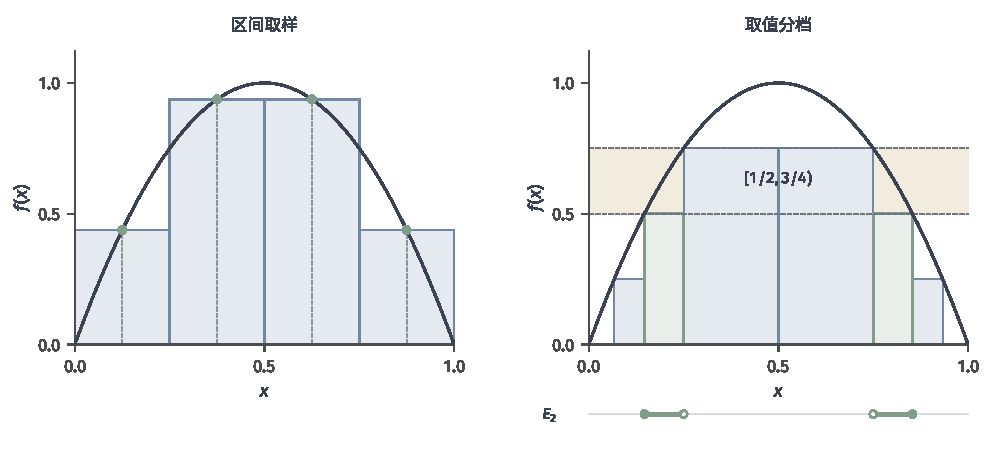
\includegraphics[width=169mm]{figures/01-mathematical-preliminaries-upper/01-mathematical-language-combinatorics-analysis-optimization/matplotlib/integral-value-layers/figure.pdf}
 \caption{对同一函数$f(x)=4x(1-x)$（$0\leq x\leq1$）作有限近似。左侧等分输入区间为四段，在中点取样形成黎曼和，矩形可高于或低于曲线。右侧将输出范围按$1/4$分档，在$E_j=\{x:j/4\leq f(x)<(j+1)/4\}$上取下界$a_j=j/4$；绿色标出$E_2=\{1/2\leq f<3/4\}$对应的两个输入区间，它们的总测度乘$1/2$给这一档的贡献。下方单独画出$E_2$并标明端点。最大值处的单点不影响积分，图中略去。左侧累计为$\sum_i f(\xi_i)\Delta x_i$，右侧简单函数的累计为$\sum_j a_jm(E_j)$。勒贝格构造加细的是取值档，权重仍来自输入集合的测度。}
 \label{fig:integral-value-layers}
\end{figure*}


\paragraph{非负勒贝格积分}
一般非负可测函数未必只取有限多个值，不能直接使用上面的有限和。
我们先保留简单函数：让它们从下方估计$f$，其积分给出能够确定的累计下界，再取全部下界的上确界作为总量。
\begin{definition}[非负勒贝格积分]
\label{def:analysis-nonnegative-lebesgue-integral}
若$f:X\to[0,\infty]$可测，定义
\begin{equation}
 \int_Xf\,\mathrm d\mu
 =\sup\left\{\int_Xs\,\mathrm d\mu:
       s\text{为非负简单函数},\ 0\leq s\leq f\right\}.
\label{eq:analysis-nonnegative-lebesgue-integral}
\end{equation}
这称为$f$关于$\mu$的非负\term{勒贝格积分}（Lebesgue integral），值可为$+\infty$。
\end{definition}
取下方积分的上确界，是为了保留所有简单函数能累计到的贡献，而不依赖某次取样。对可测$A\subseteq X$，记$\int_Af\,\mathrm d\mu=\int_Xf\mathbb I_A\,\mathrm d\mu$。在实轴上对勒贝格测度积分时，常写$\mathrm dx$代替$\mathrm dm(x)$；使用其他测度时写明$\mathrm d\mu$。

例如$f(x)=x$在$[0,1]$上的两段下方阶梯积分为$1/4$，四段时为$3/8$；等分为$n$段时，下方阶梯积分为$(n-1)/(2n)$，上方阶梯积分为$(n+1)/(2n)$，二者都趋于$1/2$。图~\ref{fig:analysis-simple-integral}用$f(x)=x^2$展示相同的逐级逼近。
\begin{figure*}[htbp]
 \centering
 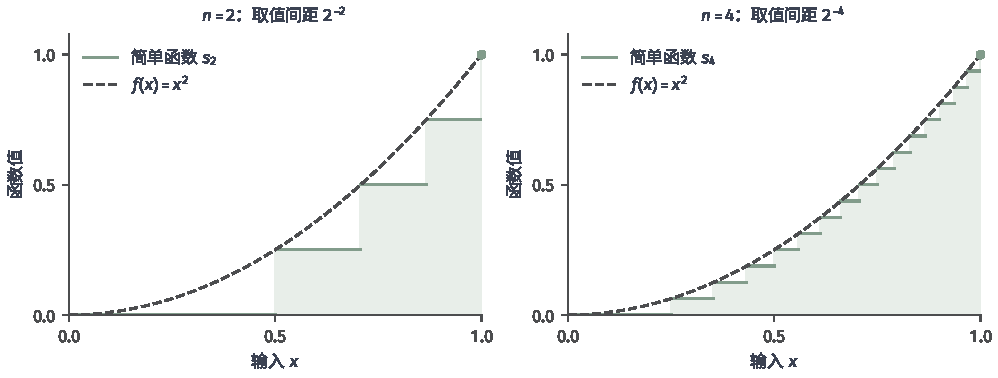
\includegraphics[width=169.0mm]{figures/01-mathematical-preliminaries-upper/01-mathematical-language-combinatorics-analysis-optimization/matplotlib/analysis-simple-integral/figure.pdf}
 \caption{$f(x)=x^2$在$[0,1]$上的简单函数逼近。图中将区间分别等分为两段、四段，在每段取函数下界，按高度乘长度求和；加细后下方累计增大，逼近积分$1/3$。简单函数还允许用一般可测集合代替图中的区间。}
 \label{fig:analysis-simple-integral}
\end{figure*}

\paragraph{可测函数的简单逼近}
上确界定义说明了怎样确定总量，还应给出实际的一列下方近似，解释任意非负可测函数如何由有限分层建立。
只加细网格会留下无穷多个取值，只截断高度又没有消除连续取值，因此同时把高度截断到$n$，再将取值向下舍入到步长$2^{-n}$的网格，得到
\begin{equation}
 \begin{aligned}
 s_n(x)&=\sum_{k=0}^{n2^n-1}\frac{k}{2^n}
  \mathbb I_{\{k/2^n\leq f<(k+1)/2^n\}}(x)\\
 &\quad+n\mathbb I_{\{f\geq n\}}(x).
 \end{aligned}
\label{eq:analysis-canonical-simple-approximation}
\end{equation}
每个$s_n$只取有限个值，取值集合可测，且$0\leq s_n\leq f$。从$n$到$n+1$时网格加细、截断高度增大，所以下方近似不减。有限$f(x)$最终低于截断高度，舍入误差小于$2^{-n}$；$f(x)=\infty$时$s_n(x)=n$。因此$s_n\uparrow f$逐点成立。这里先建立函数逼近，积分极限等式将在单调收敛定理中证明。

\paragraph{有符号勒贝格积分}
非负函数只有增加贡献的问题；有正负值时，还必须防止把两个无穷总量相减。
对实值可测$f$，令$f^+=\max\{f,0\}$、$f^-=\max\{-f,0\}$，则$f=f^+-f^-$、$|f|=f^++f^-$，正负两部分均非负可测。
只要它们的积分不同时为无穷，就定义
\[
 \int_Xf\,\mathrm d\mu=\int_Xf^+\,\mathrm d\mu-\int_Xf^-\,\mathrm d\mu.
\]
这允许单个无穷值；若两部分都为无穷，差没有定义，不能通过选择某种抵消次序给它指定一个有限勒贝格积分。

\subsubsection{可积性的要求}

可测性保证取值层可以测量；非负积分的定义保证有一个确定的扩展实数值，但都没有保证累计有限。
若要使有符号积分成为有限实数，就必须让正负两部分的总量都有限，下面用等价的绝对值积分条件统一规定。

\begin{definition}[勒贝格可积函数]
\label{def:analysis-integrable-function}
若实值可测$f$满足
\begin{equation}
 \int_X|f|\,\mathrm d\mu<\infty,
\label{eq:analysis-absolute-integrability}
\end{equation}
则称$f$关于$\mu$勒贝格可积，也称\term{绝对可积}（absolutely integrable）。其有符号勒贝格积分是有限实数。
\end{definition}
由于$f^+,f^-\leq|f|$，下方简单函数的比较保证二者的积分有限，所以这一定义确实给出有限的有符号积分。本节未附“黎曼”或“反常”限定的可积性均指这一绝对可积条件。

\paragraph{有限积分的条件}
下面分开检查“积分已经定义”和“积分取有限值”，并说明有界性还需与输入范围的测度一起判断。
非负可测函数总有定义好的非负勒贝格积分，但这个值未必有限。对有符号函数，有限积分要求正负部分都具有有限积分，等价于式~\eqref{eq:analysis-absolute-integrability}；这一等价性将在下一小节由非负积分加法正式证明。有限的有符号勒贝格积分因而必然绝对可积，不存在以正负无穷抵消得到的有限值。

若$\mu(X)<\infty$且$|f|\leq M$，由积分定义的比较关系可得$\int_X|f|\,\mathrm d\mu\leq M\mu(X)<\infty$，所以有界可测函数可积。无穷测度范围上，有界性不足，例如实轴上的常数一。无界也未必不可积，反常积分小节将算出$x^{-1/2}$在$(0,1)$上的有限积分。

\paragraph{积分与平均值}
积分不仅取决于函数和输入范围，还取决于用什么测度赋予各部分大小。
沿用前面有限加权累计的思路，取$X=\{0,1\}\subseteq\mathbb R$，设$\mu(\{0\})=1$、$\mu(\{1\})=2$，$f(0)=3$、$f(1)=-1$，则$\int_Xf\,\mathrm d\mu=1$而$\int_X|f|\,\mathrm d\mu=5$。只有在$0<\mu(X)<\infty$且$f$可积时，才能进一步定义平均值$\mu(X)^{-1}\int_Xf\,\mathrm d\mu$，本例为$1/3$。总质量为一的概率测度无需再归一化。
若同一个$X$改用勒贝格测度，两个点的长度均为零，上述函数的积分就变为零。
这与按权重$1,2$得到的$1$不矛盾，而是说明更换测度就更换了累计规则；此时总测度也为零，不能再用前面的除法定义平均值。

\subsubsection{积分的性质}
\label{sec:analysis-lebesgue-basic-properties}

定义已经给出累计值，现在要检查它是否保持加法、大小关系与集合分拆。
先从简单函数和上确界证明非负情形，再用正负分解处理有限的有符号积分；以下均指关于指定测度$\mu$的勒贝格积分。

\paragraph{非负积分的基本性质}
简单函数的积分具有线性与单调性，现在从上确界定义把这些性质推广到一般非负可测函数。证明只用前面建立的集合测度性质，为后面的累计函数和微积分基本定理提供依据。
\begin{theorem}[非负勒贝格积分的线性与单调性]
\label{lem:analysis-nonnegative-integral-properties}
设$(X,\mathcal A,\mu)$为测度空间，$f,g:X\to[0,\infty]$可测，$\alpha,\beta$为非负实数。
若$f\leq g$几乎处处，则$\int_Xf\,\mathrm d\mu\leq\int_Xg\,\mathrm d\mu$；
在$0\cdot\infty=0$的约定下，还有
\[
 \int_X(\alpha f+\beta g)\,\mathrm d\mu
 =\alpha\int_Xf\,\mathrm d\mu+\beta\int_Xg\,\mathrm d\mu.
\]
若$f=g$几乎处处且两者均可测，则它们的非负积分相同。
\end{theorem}
\begin{proof}
逐点单调性直接来自定义：每个简单函数$0\leq s\leq f$也满足$s\leq g$。
若$N$可测且$\mu(N)=0$，简单函数在$N$上的积分为零。
对$f,g$在$X\setminus N$相等的情形，将任意$0\leq s\leq f$在$N$上置零，
所得简单函数不超过$g$且积分未变。取上确界得$\int f\leq\int g$，反向相同；
几乎处处的单调性也可先作这项可测零集修改。这里不在未完备空间中任意改动后省略可测性。

对加法，任取非负简单函数$s\leq f$、$t\leq g$，简单函数的有限线性给出
$\int(f+g)\geq\int s+\int t$。分别取上确界，得到
$\int(f+g)\geq\int f+\int g$。若右侧为无穷，这已给出等式；以下设右侧有限。
反向需要检查每个下方简单函数的累计。取任意非负简单函数
$u=\sum_{j=1}^m a_j\mathbb I_{E_j}\leq f+g$，其中$a_j>0$、$E_j$两两不交，
并取规范简单逼近$s_n\uparrow f$、$t_n\uparrow g$。
固定$c\in(0,1)$，令$E_{j,n}=E_j\cap\{s_n+t_n\geq ca_j\}$。
因$s_n+t_n\uparrow f+g$且$f+g\geq a_j$于$E_j$，有$E_{j,n}\uparrow E_j$。
第~\ref{sec:analysis-set-measure-continuity}节的测度递增连续性及简单函数线性给出
\[
 \begin{aligned}
 c\int_Xu\,\mathrm d\mu
 &=\lim_n c\sum_j a_j\mu(E_{j,n})\\
 &\leq\liminf_n\left(\int_Xs_n\,\mathrm d\mu+\int_Xt_n\,\mathrm d\mu\right)\\
 &\leq\int_Xf\,\mathrm d\mu+\int_Xg\,\mathrm d\mu.
 \end{aligned}
\]
先令$c\uparrow1$，再对所有这样的$u$取上确界，便得到反向不等式。
正数倍的结论由$s\leq\alpha f$与$s/\alpha\leq f$在定义中的一一对应推出；
零数倍按约定处理，再与加法结合即得一般结论。
整个证明只使用简单函数有限和、积分上确界与集合测度连续性，没有使用一般函数的单调收敛定理。
\end{proof}

\paragraph{有符号勒贝格积分的性质}
有正负值时，实线性需要先保证所有参与相减的总量有限；绝对可积性正是这一要求。
下面同时证明可积性判别、有限线性、比较与绝对值估计。
\begin{theorem}[有符号勒贝格积分的基本性质]
\label{thm:analysis-signed-integral-properties}
设$(X,\mathcal A,\mu)$为测度空间，$f,g:X\to\mathbb R$可测。
函数$f$勒贝格可积，当且仅当$\int f^+\,\mathrm d\mu$与$\int f^-\,\mathrm d\mu$都有限。
若$f,g$勒贝格可积，$\alpha,\beta\in\mathbb R$，则$\alpha f+\beta g$也可积，且
\[
 \int_X(\alpha f+\beta g)\,\mathrm d\mu
 =\alpha\int_Xf\,\mathrm d\mu+\beta\int_Xg\,\mathrm d\mu.
\]
对上述可积的$f,g$，$f\leq g$几乎处处时有$\int f\leq\int g$，并且
\[
 \left|\int_Xf\,\mathrm d\mu\right|\leq\int_X|f|\,\mathrm d\mu.
\]
若$f$可积、$g=f$几乎处处且$g$可测，则$g$也可积，积分与$f$相同。
\end{theorem}
\begin{proof}
由$|f|=f^++f^-$及非负积分加法，
$\int|f|=\int f^++\int f^-$，所以绝对积分有限等价于正负两项均有限。
先检查有符号积分与正负分解以外的表示是否相容。若$f=u-v$，其中$u,v$非负且可积，
则$f^+,f^-\leq u+v$，故$f$可积；非负恒等式$u+f^-=v+f^+$积分后可移去有限项，得到
$\int f=\int u-\int v$。

对可积$f,g$，$|f+g|\leq|f|+|g|$保证和可积。
将$f+g=(f^++g^+)-(f^-+g^-)$代入刚才的分解结论，再用非负加法，得到
$\int(f+g)=\int f+\int g$。正数倍沿用非负缩放，负数倍交换正负部分，零数倍直接成立，因而实线性成立。
若$f\leq g$几乎处处，可积差$g-f$的积分非负，移项即得比较关系。
定义中的正负分解与实数三角不等式给出
$|\int f|\leq\int f^++\int f^-=\int|f|$。
最后，若$f=g$几乎处处且均可测，非负积分的零测修改不变性分别用于$|f|,|g|$及正负部分，便得$g$可积且积分相同。
\end{proof}

这里没有通过正负无穷抵消得到有限值。非负积分可以等于无穷，但有符号线性中的任意移项必须满足上述有限性条件。

\paragraph{零积分与零测例外}
非负函数没有正负抵消，积分为零应表示它的正值只落在零测范围内。
下面把这一判断写成等价条件，供后面比较两种积分时使用。
\begin{theorem}[非负函数的零积分判别]
\label{thm:analysis-zero-integral}
设$(X,\mathcal A,\mu)$为测度空间，$f:X\to[0,\infty]$可测，则
\[
 \int_Xf\,\mathrm d\mu=0\quad\Longleftrightarrow\quad f=0\ \text{几乎处处}.
\]
特别地，实值可测$f$满足$\int|f|\,\mathrm d\mu=0$当且仅当$f=0$几乎处处。
\end{theorem}
\begin{proof}
若积分为零，对每个正整数$k$，$f\geq k^{-1}\mathbb I_{\{f\geq1/k\}}$，故
$0\geq k^{-1}\mu(\{f\geq1/k\})$。这些集合都零测，而
$\{f>0\}=\bigcup_{k\geq1}\{f\geq1/k\}$，所以$f=0$几乎处处。
反之，非负积分的零测修改不变性将$f$与零函数的积分相等。将结论用于$|f|$便得最后一条。
\end{proof}
对有正负值的$f$，仅有$\int f=0$不能推出$f=0$几乎处处，例如$f(x)=x$在$[-1,1]$上的积分为零。

\paragraph{积分范围的可加性}
函数值可以相加，积分范围也可以分拆；后者要保持的是可测集合的不交并。
下面从测度的可数可加性直接证明这一性质，不提前使用函数列的收敛定理。
\begin{theorem}[勒贝格积分的区域可加性]
\label{thm:analysis-integral-set-additivity}
设$(X,\mathcal A,\mu)$为测度空间，$A_n\in\mathcal A$两两不交，$A=\bigcup_{n\geq1}A_n$。
若$f:X\to[0,\infty]$可测，则
\[
 \int_Af\,\mathrm d\mu=\sum_{n=1}^{\infty}\int_{A_n}f\,\mathrm d\mu,
\]
允许等式两侧为无穷。若$f$实值且在$A$上绝对可积，同一等式成立，且右侧绝对收敛。
对可测$B,C$及在$B\cup C$上绝对可积的实值$f$，还有
\[
 \int_{B\cup C}f=\int_Bf+\int_Cf-\int_{B\cap C}f.
\]
特别地，$C\subseteq B$时有$\int_{B\setminus C}f=\int_Bf-\int_Cf$。
\end{theorem}
\begin{proof}
非负积分的有限区域加法来自示性函数恒等式与非负线性。
因此$\int_A f\geq\sum_{n=1}^N\int_{A_n}f$对每个$N$成立，取部分和的上确界得到一个方向。
反向取任意简单函数$0\leq s=\sum_{j=1}^r c_j\mathbb I_{E_j}\leq f\mathbb I_A$，其中$c_j>0$且$E_j$两两不交、均包含于$A$。
测度的可数可加性及有限和与非负级数的合并给出
\[
 \int_Xs\,\mathrm d\mu
 =\sum_{j=1}^r c_j\sum_{n\geq1}\mu(E_j\cap A_n)
 =\sum_{n\geq1}\int_{A_n}s\,\mathrm d\mu
 \leq\sum_{n\geq1}\int_{A_n}f\,\mathrm d\mu.
\]
对全部这样的$s$取上确界，得到反向不等式。

若$f$在$A$上绝对可积，先对$|f|$使用非负结论，得到
$\sum_n|\int_{A_n}f|\leq\sum_n\int_{A_n}|f|=\int_A|f|<\infty$。
再分别对$f^+,f^-$使用等式并相减，便得到有符号版本。
最后，将有限实线性用于
$\mathbb I_{B\cup C}+\mathbb I_{B\cap C}=\mathbb I_B+\mathbb I_C$即得容斥式，包含情形再化为差集式。
\end{proof}
非负无穷积分的区域相加仍成立，但不能把它任意改写为含$\infty-\infty$的差。

\subsubsection{与黎曼积分的关系}

新的定义既要处理原来无法累计的函数，也要与已有数值相容。下面先证明黎曼可积函数没有被改变，再说明零测改值为什么使两种可积范围分开。


\paragraph{黎曼积分与勒贝格积分的关系}
改变累计方式之后，必须检验原来已经能够计算的积分是否得到保留。
下面将黎曼上下和看作简单函数的积分，以可测包络和零测余量证明两种积分一致。
\begin{theorem}[黎曼积分与勒贝格积分的一致性]
\label{thm:analysis-riemann-lebesgue-consistency}
设$a<b$，$f:[a,b]\to\mathbb R$有界且黎曼可积。
则$f$勒贝格可测、勒贝格可积，且
\[
 \int_a^bf(x)\,\mathrm dx\ \text{（黎曼）}
 =\int_{[a,b]}f\,\mathrm dm\ \text{（勒贝格）}.
\]
反向蕴含不成立：有界勒贝格可积函数未必黎曼可积。
\end{theorem}
\begin{proof}
设$|f|\leq M$在$[a,b]$上黎曼可积。由Darboux判据，可取一列分割$P_n$，后一个是前一个的加细，并使$U(f,P_n)-L(f,P_n)<1/n$。
在$P_n$的每个小区间内部，令下阶梯函数$\ell_n$取该段的下确界$m_i$，上阶梯函数$u_n$取上确界$M_i$；
有限个分割点上的取值不影响积分，可以都取$f$的值。于是$\ell_n\leq f\leq u_n$，它们都是简单函数，
且$\int\ell_n\,\mathrm dx=L(f,P_n)$、$\int u_n\,\mathrm dx=U(f,P_n)$。加细使$\ell_n$逐点不减、$u_n$逐点不增。
令$\ell=\sup_n\ell_n$、$u=\inf_nu_n$。它们可测，因为$\{\ell>c\}=\bigcup_n\{\ell_n>c\}$是可数个可测集合的并，$u$同理；并且$\ell\leq f\leq u$。
非负可测函数$u-\ell$对每个$n$都满足$u-\ell\leq u_n-\ell_n$，由积分的单调性，
\[
 0\leq\int_{[a,b]}(u-\ell)\,\mathrm dx\leq U(f,P_n)-L(f,P_n)<\frac1n,
\]
所以这个积分为零。由定理~\ref{thm:analysis-zero-integral}，$\{u\neq\ell\}$是零测集。$f$只在这个零测集上可能与可测函数$\ell$不同，
而勒贝格测度完备，零测集的任意子集都可测，所以$f$勒贝格可测。有限区间上的有界可测函数绝对可积，故可使用有符号积分的比较关系。
最后，每个$n$都有$L(f,P_n)=\int\ell_n\leq\int f\leq\int u_n=U(f,P_n)$（有符号情形先给$f$加常数$M$使之非负，再用有限线性移去常数），
两端都趋于黎曼积分，所以勒贝格积分等于黎曼积分。

狄利克雷函数是有界勒贝格可积却不黎曼可积的反例，证明了反向蕴含不成立。
\end{proof}

\paragraph{黎曼可积性的测度判据}
一致性定理保留了已有积分，却还没有回答哪些勒贝格可积函数同时黎曼可积。
下面将上下和误差与不连续点的测度联系起来，给出有界函数的准确判据。
\begin{theorem}[黎曼可积性的勒贝格判据]
\label{thm:analysis-riemann-lebesgue-criterion}
设$a<b$，$f:[a,b]\to\mathbb R$有界，$D$为$f$相对于$[a,b]$的不连续点集。
则$D$勒贝格可测，并且$f$黎曼可积当且仅当$m(D)=0$。
\end{theorem}
\begin{proof}
先用局部振幅描述不连续。记$I_r(x)=[a,b]\cap(x-r,x+r)$，定义
\[
 \omega_f(x)=\inf_{r>0}\left(\sup_{I_r(x)}f-\inf_{I_r(x)}f\right).
\]
由于$x\in I_r(x)$，$\omega_f(x)=0$恰好表示在足够小的邻域内所有取值都接近$f(x)$，因此等价于$f$在$x$连续。
对$t>0$，记$D_t=\{x:\omega_f(x)\geq t\}$。
若$\omega_f(x)<t$，存在一个邻域，其上振幅小于$t$；该邻域内充分靠近$x$的点也有更小的邻域包含于其中，所以也不属于$D_t$。
因此$D_t$在$[a,b]$中闭，进而紧；$D=\bigcup_{k\geq1}D_{1/k}$为Borel集。

若$f$黎曼可积，给定$t,\varepsilon>0$，取分割$P$使$U(f,P)-L(f,P)<t\varepsilon$。
除有限个分割点外，$D_t$中的每点都位于某个振幅至少为$t$的小区间内。
这些小区间的总长度不超过$(U-L)/t<\varepsilon$，分割点自身零测，故$m(D_t)<\varepsilon$。
由$\varepsilon$任意得$m(D_t)=0$，再取可数并得到$m(D)=0$。

反之，设$m(D)=0$且$|f|\leq M$；$M=0$时结论直接成立，以下取$M>0$。
给定$\varepsilon>0$，先取$t>0$使$t(b-a)<\varepsilon/2$。
紧零测集$D_t$可由开集$O$包住，使$m(O)<\varepsilon/(4M)$。
每个$x\notin D_t$都有一个相对开邻域$V_x$，其上$f$的振幅小于$t$。
$O$与这些$V_x$覆盖$[a,b]$，取一个有限子覆盖。
由式~\eqref{eq:analysis-cover-uniform-radius}，这个覆盖存在共同半径$r>0$，使每点的相对$r$球包含在某个覆盖成员内。取$\delta=r$，长度小于$\delta$的子区间就落在以其中一点为中心的$r$球内，因此也落在某个覆盖成员内。

取细度小于$\delta$的分割。能落在某个$V_x$内的小区间，振幅小于$t$；其余小区间都包含于$O$，总长度不超过$m(O)$，振幅至多$2M$。
因此
\[
 U(f,P)-L(f,P)\leq t(b-a)+2M m(O)<\varepsilon.
\]
由Darboux判据，$f$黎曼可积。
\end{proof}

\paragraph{零测集上的改值}
前面的累计按可测块的测度赋权，因而只落在可测零测集上的贡献为零。
保持可测性的零测修改不改变勒贝格积分，这已在定理~\ref{lem:analysis-nonnegative-integral-properties}及定理~\ref{thm:analysis-signed-integral-properties}中证明。这里用它比较两种可积范围，而不再从简单函数重新推导。
在勒贝格测度下，完备性保证任意零测子集仍可测，所以零测范围内任意有限实值改动都保持可测性。
若采用未完备的一般测度空间，则不能省略修改后仍可测的条件。
狄利克雷函数与零函数的关系正是这个机制的实例。

这种修改可能破坏黎曼可积性。零函数在可数稠密集$\mathbb Q\cap[0,1]$上改为一，就变为不黎曼可积的狄利克雷函数。因此黎曼可积性判据要求原函数几乎处处连续，不能替换成“几乎处处等于一个连续函数”。有限个点的有限改值仍保持黎曼可积，修改前后的积分才仍相等。

\subsection{不定积分和变上限积分}
\label{sec:analysis-definite-indefinite-integrals}

定积分在指定范围上给出一个数；寻找导数等于给定函数的原函数，则产生一个函数族。把定积分的上端点设为变量也会得到一个函数，下面先分别定义这两种对象，暂不把它们认定为同一对象。

\subsubsection{不定积分}

这里暂时从累计转回求导问题：给定$f$，寻找导数为$f$的函数。先独立定义这个对象，才能在基本定理中真正证明它与积分的联系。


\paragraph{原函数}
对已知$f$寻找满足$G'=f$的可微函数$G$，称为求原函数。原函数的定义只涉及求导，还没有断言它与定积分有何关系。例如$x^2/2$是$x$在实轴上的一个原函数。

\paragraph{不定积分}
若$f$在区间$I$上有一个原函数$G$，则其全部原函数写为$G+C$，其中$C$为任意实常数，记作$\int f(x)\,\mathrm dx=G(x)+C$，称为不定积分。两个原函数之差的导数为零，由中值定理，它们在区间上只差常数；如果定义域由分离的区间组成，每段可以有不同常数。不定积分表示一个函数族，区别于固定上下限后得到的数值。

\subsubsection{变上限积分}

将固定范围上的积分改为随端点变化的累计，可以得到一个新函数；它的存在来自各子区间可积，尚不等于它已经是原函数。


\paragraph{变上限积分}
若$f$在$[a,b]$上黎曼可积，令
\[
 F(x)=\int_a^xf(t)\,\mathrm dt,\qquad a\leq x\leq b.
\]
得到的$F$称为变上限积分函数，也称累计函数。$t$是积分变量，$x$是函数的自变量。比如$f(t)=1$时，$F(x)=x-a$。变上限积分是否可导、是否以$f$为导数，需要由微积分基本定理判断，不能直接从记号得出。

\paragraph{变上限勒贝格积分}
若$f$在$[a,b]$上勒贝格可积，同样定义$F(x)=\int_a^xf(t)\,\mathrm dt$，此时积分按勒贝格定义计算。可积性保证每个子区间上的积分有限，前面的区域分拆给出$F(y)-F(x)=\int_x^yf$；有界黎曼可积函数的两种累计函数相同。对一般可积函数，累计函数是否处处或几乎处处可导，需要另外证明。

\subsubsection{原函数与累计函数的关系}

原函数从求导关系定义，累计函数从定积分构造；记号相似没有证明二者等价。若$f$连续，下一小节将证明累计函数是它的原函数；若$f$仅勒贝格可积，能一般地保证的是几乎处处恢复$f$。例如阶跃函数可以累计，却不可能在跳跃点附近处处等于某个函数的导数，这一差别将在基本定理中具体检验。

\subsection{微积分基本定理}
\label{sec:measurable-differentiation-recovery}
\label{sec:analysis-fundamental-calculus}

求导记录局部变化，积分记录一段范围内的累计，二者能否相互恢复要分别回答两个问题。
第一，给定函数$G$，积分其导数能否得到$G(b)-G(a)$；第二，给定被积函数$f$，对累计函数$F(x)=\int_a^xf$求导能否恢复$f(x)$。
前者检查总变化是否全部由导数记录，后者检查局部平均是否能识别点值。下面分别说明黎曼与勒贝格条件，不将“处处”与“几乎处处”的结论混在一起。

\subsubsection{导数的积分}

先给定$G$再计算其导数的积分，目标是恢复端点变化。
连续导数提供最直接的充分条件；导数仅黎曼可积时仍可恢复，而只知道几乎处处可导且导数勒贝格可积，还需要对$G$的整体变化加条件。

\paragraph{黎曼可积导数的基本定理}
中值定理把每段端点增量写成导数取样值乘区间长度，因此端点恢复的关键是这些取样和能否趋于积分，而不必要求导数连续。
下面先给出黎曼可积导数的结论；连续导数是其中自动满足可积性的特例。
\begin{theorem}[黎曼可积导数的端点公式]
\label{thm:analysis-riemann-derivative-ftc}
\label{thm:analysis-newton-leibniz-continuous}
设$G$在$[a,b]$上连续、在$(a,b)$上可导，且存在黎曼可积函数$g:[a,b]\to\mathbb R$在内点满足$g=G'$。
则
\[
 \int_a^bg(x)\,\mathrm dx=G(b)-G(a).
\]
端点处给$g$指定的有限值不影响积分。特别地，若$G\in C^1([a,b])$，可取$g=G'$。
上述黎曼积分也等于相应的勒贝格积分。
\end{theorem}
\begin{proof}
对任意分割，在每个小区间上用中值定理选$\xi_i$，得到
\[
 G(b)-G(a)=\sum_i\bigl(G(x_i)-G(x_{i-1})\bigr)
 =\sum_i g(\xi_i)(x_i-x_{i-1}).
\]
$g$黎曼可积保证任意细分割的这些取样和都趋于$\int_a^bg$，所以等式成立。
改变两个端点的值仍保持黎曼可积且不改变积分。若$G\in C^1([a,b])$，连续函数的黎曼可积性保证可选$g=G'$；两种积分的一致性由定理~\ref{thm:analysis-riemann-lebesgue-consistency}给出。
\end{proof}

\paragraph{康托尔函数}
\label{sec:analysis-cantor-function}
几乎处处可导只记录了零测例外之外的局部变化，未必记录全部端点变化。下面的函数连续且几乎处处导数为零，但从$0$到$1$仍增加了$1$。

第~\ref{sec:analysis-cantor-set}节已构造康托尔集$C$并证明它为零测集。现在利用同一删除过程定义一个函数：每一步位于左、右保留区间，分别确定三进制表示的下一位为$0$、$2$，所以$C$中每点都能选只含这两个数字的表示
\[
 x=\sum_{j=1}^\infty\frac{\varepsilon_j}{3^j},\qquad
 F(x)=\sum_{j=1}^\infty\frac{\varepsilon_j/2}{2^j},
 \qquad\varepsilon_j\in\{0,2\}.
\]
第二个几何控制的级数把三进制数字$0,2$分别改为二进制数字$0,1$；$x=1$取全为$2$的表示。若$C$中两点的三进制位首次在第$k$位不同，较大点的二进制主位增加$2^{-k}$，而后续位造成的反向差至多为$\sum_{j>k}2^{-j}=2^{-k}$，所以$F$不减。每个删去区间的两端分别对应某一二进制位为$0$而后全为$1$、该位为$1$而后全为$0$，这条尾和恒等式又保证两值相等。例如$1/3=0.0222\ldots_3$与$2/3=0.2000\ldots_3$都对应$1/2$。在该开区间上把$F$定义为这个共同值，就得到整个$[0,1]$上的\term{康托尔函数}（Cantor function）。

这个函数非减，$F(0)=0,F(1)=1$。在第$n$步的每个保留区间上，它的全部变化不超过$2^{-n}$；删去区间上则不变化。两个相距小于$3^{-n}$的点之间至多涉及两个第$n$步保留区间，因而函数值之差不超过$2^{1-n}$；先选$n$再取输入误差$\delta=3^{-n}$，就得到一致连续性。每个删去的开区间内$F$恒定，所以$F'=0$于$[0,1]\setminus C$，即几乎处处成立；在导数未定义的零测例外上置零，则
\[
 F(1)-F(0)=1,\qquad \int_0^1F'(x)\,\mathrm dx=0.
\]
它不绝对连续：第$n$步保留区间总长度为$(2/3)^n$，但各区间端点变化的总和仍为$2^n2^{-n}=1$。这既解释了绝对连续假设的作用，也说明“连续、几乎处处可导、导数可积”三项合在一起仍不足以由导数积分恢复函数。

\paragraph{绝对连续函数的导数基本定理}
康托尔函数说明，连续性不能排除集中在零测集上的整体变化，因而需要更强的条件。
定义~\ref{def:measurable-absolutely-continuous-function}的绝对连续条件控制许多短区间上的总变化，能排除导数遗漏整体变化的情形。
\begin{theorem}[绝对连续函数的导数积分]
\label{thm:measurable-absolute-continuity-ftc}
若$G:[a,b]\to\mathbb R$绝对连续，则$G'$几乎处处存在，并有实值勒贝格可积函数$g$与$G'$几乎处处相等，使每个$x\in[a,b]$满足
\begin{equation}
 G(x)=G(a)+\int_a^xg(t)\,\mathrm dt.
\label{eq:measurable-absolute-continuity-representation}
\end{equation}
特别地，$G(b)-G(a)=\int_a^bG'(t)\,\mathrm dt$，其中在未定义导数的零测例外上可取值零；这些积分为勒贝格积分。
\end{theorem}
绝对连续性推出几乎处处可导和上述积分表示，是这里引用的测度论基本结论，完整证明见教材\scite{math-folland1999real}。
这项引用包括导数的存在、可积性与端点恢复，不能用已经知道导数存在来代替。
另一个方向——勒贝格可积函数的累计必绝对连续——将在“积分的导数”中直接证明，因此两种描述的等价性仍会建立。

\paragraph{局部Lipschitz连续函数的导数基本定理}
如果用Lipschitz条件控制函数的变化，就能通过绝对连续性保证几乎处处导数存在，并在闭区间上由导数积分恢复总变化。\term{Rademacher定理}（Rademacher theorem）保证例外点只占零测集。
\begin{theorem}[一维Rademacher定理]
\label{thm:measurable-rademacher}
若$U\subseteq\mathbb R$为开集，$f:U\to\mathbb R$局部Lipschitz连续，则$f'$在$U$内几乎处处存在且有限。若$f$在某个开区间上具有Lipschitz常数$L$，则该区间内导数存在的点满足$|f'|\leq L$。
\end{theorem}
这里的导数存在性将通过绝对连续函数基本定理得到，还需用可数覆盖把局部结论合并到整个开集。
\label{sec:analysis-rademacher-proof}
\begin{proof}
紧区间上的Lipschitz函数绝对连续，基本定理便保证它几乎处处可导。若$f$只在开集$U$上局部Lipschitz，可选取可数多个端点为有理数的闭区间，使其内部覆盖$U$，并使每个区间都包含在某个具有Lipschitz常数的邻域内。
各区间上的不可导点集为零测集，它们的可数并仍为零测集，故$f'$在$U$内几乎处处存在。导数存在的点处，Lipschitz差商界取极限便给出$|f'|\leq L$。
\end{proof}
绝对值函数在原点的左右导数不同，仍符合上述几乎处处结论；定理没有把尖点处的左右导数合成一个经典导数。

在闭区间上具有Lipschitz常数的函数绝对连续，因此其导数除几乎处处存在之外，还可用勒贝格积分恢复端点变化。
连续、几乎处处可导、导数可积三项合在一起则不充分，康托尔函数已给出反例。

\subsubsection{积分的导数}

现在改为先给定$f$，再构造累计函数$F(x)=\int_a^xf(t)\,\mathrm dt$。
差商是一个短区间上的平均。下面按被积函数的条件区分三种情况：黎曼可积时先在连续点恢复，局部勒贝格可积时在几乎每一点恢复，闭区间上勒贝格可积时还得到整个区间上的绝对连续性。

\paragraph{黎曼可积函数}
累计函数的增量来自一个短区间，把它除以区间长度后，能否恢复点值取决于该点附近的取值变化。
下面只在要恢复的点要求连续，不额外要求全区间连续。
\begin{theorem}[黎曼累计函数在连续点的导数]
\label{thm:analysis-riemann-primitive-derivative}
设$f$在$[a,b]$上黎曼可积，$F(x)=\int_a^xf(t)\,\mathrm dt$。
若$f$在$c\in(a,b)$处连续，则$F'(c)=f(c)$；端点连续时对应单侧导数也等于端点值。
特别地，若$f$在$[a,b]$上连续，则$F\in C^1([a,b])$且$F'=f$。
\end{theorem}
\begin{proof}
由区间可加性与有限线性，对非零小增量$h$有
\[
 \frac{F(c+h)-F(c)}h-f(c)
 =\frac1h\int_c^{c+h}(f(t)-f(c))\,\mathrm dt.
\]
右侧绝对值不超过$c$与$c+h$之间的$\sup|f(t)-f(c)|$，连续性使它趋零。
对端点只取允许方向的$h$。若$f$处处连续，则所得导数$f$也连续，即$F\in C^1([a,b])$。
\end{proof}

由黎曼可积性的测度判据，不连续点组成零测集，因此这里也得到$F'=f$几乎处处。不能将结论加强为处处成立：阶跃函数$\mathbb I\{x\geq0\}$的累计函数在跳跃点不可导。

\paragraph{局部勒贝格可积函数}
研究某一点附近的平均累计，只需要附近紧范围上的绝对积分有限，不必要求整个定义域的积分有限。
若可测函数$f$在实轴开集$U$内的每个紧子集$K$上都满足$\int_K|f|\,\mathrm dx<\infty$，称$f$局部勒贝格可积。它只要求局部范围内绝对可积，允许整个无界定义域上的绝对积分为无穷。

连续点处的短区间平均趋于函数值。对局部可积函数，\term{Lebesgue微分定理}（Lebesgue differentiation theorem）将这一结论推广到几乎每一点\scite{math-hunter2011measure}。
\begin{theorem}[一维Lebesgue微分定理]
\label{thm:measurable-lebesgue-differentiation}
若$f$在开集$U\subseteq\mathbb R$上局部勒贝格可积，则对几乎每个$x\in U$，
\begin{equation}
 \lim_{r\downarrow0}\frac1{2r}\int_{x-r}^{x+r}|f(t)-f(x)|\,\mathrm dt=0.
\label{eq:measurable-lebesgue-point}
\end{equation}
从而$(2r)^{-1}\int_{x-r}^{x+r}f(t)\,\mathrm dt\to f(x)$。
\end{theorem}
满足式~\eqref{eq:measurable-lebesgue-point}的点称为勒贝格点；定理中的积分均为勒贝格积分。第二条由平均差的绝对值不超过平均绝对差得到。第一条的一般证明需要覆盖估计，本节引用其结论，不把连续点的证明充当一般证明。


在$U$中的一个开区间$I$上固定$x_0\in I$，令$F(x)=\int_{x_0}^xf(t)\,\mathrm dt$。
任意$x\in I$与$x_0$之间的闭区间都是$U$的紧子集，所以积分有限；这里下限不必取在定义域端点。
在$f$的内点勒贝格点$x$，区间可加性给出
\[
 \begin{aligned}
 \left|\frac{F(x+h)-F(x)}h-f(x)\right|
 &\leq\frac1{|h|}\int_{\min\{x,x+h\}}^{\max\{x,x+h\}}|f(t)-f(x)|\,\mathrm dt\\
 &\leq\frac1{|h|}\int_{x-|h|}^{x+|h|}|f(t)-f(x)|\,\mathrm dt.
 \end{aligned}
\]
最后一项是式~\eqref{eq:measurable-lebesgue-point}中平均绝对差的两倍，因而趋零。
所以$F'(x)=f(x)$在每个勒贝格点成立，特别地在$I$上几乎处处成立。
局部可积不能保证靠近定义域端点的累计有限：例如$f(t)=1/t$在$(0,1)$上局部可积，$\int_{1/2}^xf(t)\,\mathrm dt$对每个$x\in(0,1)$有意义，但不能把下限改为$0$而仍要求有限。


\paragraph{勒贝格可积函数}
若进一步要求$f$在整个闭区间$[a,b]$上勒贝格可积，则端点累计也有限，而且小测度集合上的积分可以统一控制。
这使累计函数在整个$[a,b]$上绝对连续；导数结论仍是前一种情形给出的勒贝格点处恢复。
\begin{theorem}[勒贝格累计函数的绝对连续性与导数]
\label{thm:analysis-lebesgue-primitive-derivative}
若$f:[a,b]\to\mathbb R$勒贝格可积，令$F(x)=\int_a^xf(t)\,\mathrm dt$，则$F$绝对连续。
在$f$的每个内点勒贝格点处，$F'(x)=f(x)$；特别地，
\begin{equation}
 F'(x)=f(x)\quad\text{几乎处处成立}.
\label{eq:measurable-indefinite-integral-derivative}
\end{equation}
这里全部使用勒贝格积分。
\end{theorem}
\begin{proof}
先控制小测度集合上的累计。给定$\varepsilon>0$，由非负积分的上确界定义，选有界简单函数$0\leq s\leq|f|$使
$\int(|f|-s)<\varepsilon/2$，并记$s\leq M$。
对可测$E$，积分的比较与有限加法给出
\[
 \int_E|f|\,\mathrm dm\leq M m(E)+\varepsilon/2.
\]
取$\delta>0$使$M\delta<\varepsilon/2$（$M=0$时任取$\delta$），则$m(E)<\delta$使该积分小于$\varepsilon$。
若$(a_j,b_j)$为有限个两两不交区间，$\sum_j(b_j-a_j)<\delta$，令$E$为它们的并，区域可加性与绝对值界给出
\[
 \sum_j|F(b_j)-F(a_j)|\leq\sum_j\int_{a_j}^{b_j}|f(t)|\,\mathrm dt
 =\int_E|f|\,\mathrm dm<\varepsilon.
\]
这就是$F$绝对连续；有限端点不影响勒贝格积分。

将$f$限制到$(a,b)$，它局部勒贝格可积。前面的差商估计已经证明，在每个内点勒贝格点处$F'=f$，Lebesgue微分定理保证这些点占据几乎整个区间。
小集合估计只使用前面的积分性质，不依赖后面的函数列收敛定理。
\end{proof}

合看两个方向的基本定理，在$[a,b]$上，$F$绝对连续当且仅当存在勒贝格可积函数$g$使
$F(x)=F(a)+\int_a^xg(t)\,\mathrm dt$，此时$F'=g$几乎处处。
正向由定理~\ref{thm:measurable-absolute-continuity-ftc}给出，反向及几乎处处求导由刚才的定理给出。
这说明绝对连续为何适合恢复整体变化；康托尔反例则说明一致连续还不够。
同时，几乎处处恢复不能加强为逐点恢复：狄利克雷函数的累计恒为零，导数处处为零，却在有理点与指定的被积函数值不同。

图~\ref{fig:analysis-process-accumulation-increment}将短区间上的面积，与累计函数的增量放在同一组端点下比较。
\begin{figure*}[!htbp]
 \centering
 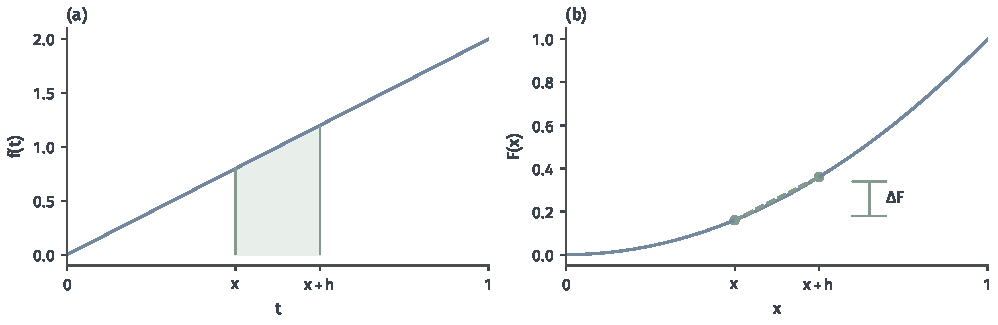
\includegraphics[width=169.0mm]{figures/01-mathematical-preliminaries-upper/01-mathematical-language-combinatorics-analysis-optimization/matplotlib/chapter3-concept-processes/accumulation-increment.pdf}
 \caption{(a) $f(t)=2t$在$[x,x+h]$上的绿色面积。(b) $F(x)=x^2$对应的增量$\Delta F$。图取$x=0.4,h=0.2$，两者都等于$0.2$。将增量除以$h$得到短区间平均值；只有再令$h\to0$，它才趋于$f(x)$，不能把有限平均值直接当作基点导数。}
 \label{fig:analysis-process-accumulation-increment}
\end{figure*}

\subsection{积分的运算法则}
\label{sec:analysis-integral-calculus-rules}

从这里起，本章后续的积分一律采用勒贝格积分；“可积”指绝对值积分有限，非负函数的积分则允许为无穷。
前面已经证明积分的基本性质，现在说明如何用它们计算函数加减、范围分拆、换元与分部积分。

\subsubsection{积分的基本运算}

函数相加与积分范围相加是不同的操作，分别由线性和区域可加性保证。
计算时先检查可测性及绝对可积性，再使用相应等式；正负无穷不能通过移项抵消。

\paragraph{和的积分}
在同一测度空间$(X,\mathcal A,\mu)$上，若实值函数$f,g$均可积，则$|f+g|\leq|f|+|g|$保证$f+g$可积。
定理~\ref{thm:analysis-signed-integral-properties}给出
\[
 \int_X(f+g)\,\mathrm d\mu=\int_Xf\,\mathrm d\mu+\int_Xg\,\mathrm d\mu.
\]
反方向也可将同一范围、同一测度下的两个有限积分合并为和的积分。

\paragraph{差的积分}
两个可积函数的差仍可积，因为$|f-g|\leq|f|+|g|$。同一线性定理给出
\[
 \int_X(f-g)\,\mathrm d\mu=\int_Xf\,\mathrm d\mu-\int_Xg\,\mathrm d\mu.
\]
这里两项都是有限实数，不涉及正负无穷的相减。

\paragraph{数乘的积分}
把被积函数乘以固定实数$c$，积分也乘以$c$。若$f$可积，则$cf$可积，且
\[
 \int_Xcf\,\mathrm d\mu=c\int_Xf\,\mathrm d\mu.
\]
这仍是定理~\ref{thm:analysis-signed-integral-properties}的特例；$c=0$时两侧都为零。

\paragraph{积的积分}
乘积需要另行检查可积性，不能直接套用线性。若$f$可积、$g$可测且$|g|\leq M$几乎处处，其中$M$为有限常数，则$|fg|\leq M|f|$保证$fg$可积。
但即使$f,g,fg$都可积，也不能把乘积的积分拆成两个积分相乘：例如在$[0,1]$上取$f(x)=g(x)=x$，则$\int_0^1fg=1/3$，而$(\int_0^1f)(\int_0^1g)=1/4$。

\paragraph{不交范围的积分}
同一函数在不同范围上的累计，可以用区域可加性分拆。
若$A,B\in\mathcal A$、$A\cap B=\varnothing$，且$f$在$A\cup B$上可积，则定理~\ref{thm:analysis-integral-set-additivity}给出
\[
 \int_{A\cup B}f\,\mathrm d\mu=\int_Af\,\mathrm d\mu+\int_Bf\,\mathrm d\mu.
\]
这与“和的积分”不同：这里改变积分范围，被积函数没有相加。

\paragraph{重叠范围的积分}
若两个范围重叠，分别累计会把交集计算两次，需要减去一次。
对可测$A,B$及在$A\cup B$上可积的$f$，有
\[
 \int_{A\cup B}f\,\mathrm d\mu
 =\int_Af\,\mathrm d\mu+\int_Bf\,\mathrm d\mu-\int_{A\cap B}f\,\mathrm d\mu.
\]
将$A\cup B$拆成$A\setminus B$、$A\cap B$、$B\setminus A$三个不交部分，再用区域可加性即可得到此式。

\paragraph{差集上的积分}
从可测范围$A$中去掉可测子集$B\subseteq A$时，去掉的累计量正是$B$上的积分。
若$f$在$A$上可积，由$A=(A\setminus B)\cup B$的不交分拆，得到
\[
 \int_{A\setminus B}f\,\mathrm d\mu=\int_Af\,\mathrm d\mu-\int_Bf\,\mathrm d\mu.
\]

\paragraph{区间的分拆与方向}
在实轴的勒贝格测度下，有限个端点不影响积分，因而可以在一个中间点拆分区间。
若$f$在$[a,b]$上可积、$a\leq c\leq b$，则
\[
 \int_a^bf(x)\,\mathrm dx=\int_a^cf(x)\,\mathrm dx+\int_c^bf(x)\,\mathrm dx.
\]
区间记号另采用有向约定$\int_b^af=-\int_a^bf$，并令$\int_a^af=0$；普通可测集合上的积分没有这一方向约定。

\paragraph{积分的比较}
被积函数几乎处处的大小关系可以传给积分。若$f,g$可积且$f\leq g$几乎处处，则
\[
 \int_Xf\,\mathrm d\mu\leq\int_Xg\,\mathrm d\mu.
\]
因为$g-f$非负且可积，其积分非负，再由差的积分公式移项即可。

\paragraph{积分的绝对值界}
累计中的正负抵消不会超过绝对值的累计。由$-|f|\leq f\leq|f|$及积分比较得到
\[
 \left|\int_Xf\,\mathrm d\mu\right|\leq\int_X|f|\,\mathrm d\mu.
\]
此处$f$可积，所以不等式两侧均有限。

\paragraph{积分的误差估计}
将绝对值界用于两个可积函数之差，就能控制积分结果的误差：
\[
 \left|\int_Xf\,\mathrm d\mu-\int_Xg\,\mathrm d\mu\right|
 \leq\int_X|f-g|\,\mathrm d\mu.
\]
若进一步有$\mu(X)<\infty$且$|f-g|\leq\eta$几乎处处，则右侧不超过$\eta\mu(X)$。
后面的极限与积分问题将用这一估计，把函数的共同误差转成积分误差。

\subsubsection{换元积分法}
\label{sec:analysis-coordinate-change-integral-applications}

变量替换既改变函数表达，也改变输入集合的测度，导数的绝对值负责一维长度的缩放。
下面使用一一对应的换元，先给可测函数的结论，再说明有向端点的写法。

\paragraph{可测函数的换元公式}
对非负函数，换元要保留全部累计；对有符号函数，还需保证正负部分都有限。
下面用微分同胚条件同时控制可逆性、可测性与局部长度变化。
\begin{theorem}[一维勒贝格积分的换元公式]
\label{thm:analysis-lebesgue-change-variables}
设$I,J\subseteq\mathbb R$为开区间，$T:I\to J$是$C^1$微分同胚，即$T$双射且$T,T^{-1}$连续可微。
对非负勒贝格可测$g:J\to[0,\infty]$，有
\[
 \int_Jg(u)\,\mathrm du=\int_Ig(T(x))|T'(x)|\,\mathrm dx,
\]
允许两边为无穷。若$g:J\to\mathbb R$可测，则$g$在$J$上可积当且仅当$g\circ T\,|T'|$在$I$上可积，此时同一等式给出有限积分值。
\end{theorem}
一般换元定理的证明先将局部长度关系推广到可测集合，再经简单函数及单调逼近推广到非负函数；这里引用这一结论\scite{math-folland1999real}。
有符号版本由先对$|g|$换元、确认绝对可积，再分别对正负部分换元得到。

\paragraph{有向区间的换元}
若$[a,b]\subset I$且$g$在$T([a,b])$上可积，$T$在整个区间严格单调，普通长度累计与有向端点可分别写为
\[
 \int_{T([a,b])}g(u)\,\mathrm du
 =\int_a^b g(T(x))|T'(x)|\,\mathrm dx,
 \qquad
 \int_{T(a)}^{T(b)}g(u)\,\mathrm du
 =\int_a^b g(T(x))T'(x)\,\mathrm dx.
\]
第一式按像区间从左到右累计，第二式的方向保留在端点和$T'$中；两式仍是勒贝格积分。
例如$T(x)=2x$把$[0,1]$变为$[0,2]$，故$\int_0^2u^2\,\mathrm du=\int_0^1(2x)^2\,2\,\mathrm dx=8/3$。

\subsubsection{分部积分法}
\label{sec:analysis-integration-remainders}

乘积求导把两个导数项联系起来，绝对连续函数的端点恢复公式允许积分后把其中一项移到另一侧。
下面直接使用绝对连续条件；连续可微函数是其特例。

\paragraph{分部积分公式}
绝对连续保证导数几乎处处存在、可积且记录全部增量，因此能够给乘积求导式积分。
只知道几乎处处可导仍不充分，前面的康托尔函数已说明这一差别。
\begin{theorem}[勒贝格积分的分部积分公式]
\label{thm:analysis-lebesgue-integration-by-parts}
若$u,v:[a,b]\to\mathbb R$绝对连续，则$uv$绝对连续，$uv'$与$u'v$可积，且
\begin{equation}
 \int_a^bu(x)v'(x)\,\mathrm dx
 =[u(x)v(x)]_a^b-\int_a^bu'(x)v(x)\,\mathrm dx.
\label{eq:analysis-integration-by-parts}
\end{equation}
导数在零测例外上的可测有限取值不影响结果。
\end{theorem}
\begin{proof}
$u,v$连续且有界，导数可积，所以$uv'$与$u'v$可积。
对有限个两两不交区间，有
\[
 \begin{aligned}
 \sum_j|u(b_j)v(b_j)-u(a_j)v(a_j)|
 &\leq\|u\|_\infty\sum_j|v(b_j)-v(a_j)|\\
 &\quad+\|v\|_\infty\sum_j|u(b_j)-u(a_j)|.
 \end{aligned}
\]
两因子的绝对连续性使右侧随区间总长度趋零，故$uv$绝对连续。
在两导数都存在的点，$(uv)'=u'v+uv'$；将绝对连续函数的端点恢复定理用于$uv$，再用有限线性移项，便得公式。
\end{proof}
例如取$u(x)=x$、$v(x)=e^x$，得到$\int_0^1xe^x\,\mathrm dx=[xe^x]_0^1-\int_0^1e^x\,\mathrm dx=1$。
在无穷区间上使用时，先对有限截断应用公式，再分别核查边界项的极限以及两个被积项的绝对可积性，不能无故删除端点项。

\paragraph{Taylor公式的积分余项}
分部积分还能给出Taylor展开的积分余项。设$f$在连接$x_0$和$x_0+h$的线段邻域内
$r+1$阶连续可微，其中$r$为非负整数，令$\phi(t)=f(x_0+th)$。
记
\[
 I_r=\frac1{r!}\int_0^1(1-t)^r\phi^{(r+1)}(t)\,\mathrm dt.
\]
基本定理给出$I_0=\phi(1)-\phi(0)$；对$r\geq1$分部积分，
\[
 I_r=-\frac{\phi^{(r)}(0)}{r!}
       +\frac1{(r-1)!}\int_0^1(1-t)^{r-1}\phi^{(r)}(t)\,\mathrm dt
     =-\frac{\phi^{(r)}(0)}{r!}+I_{r-1}.
\]
逐次代入并用$\phi^{(k)}(0)=h^k f^{(k)}(x_0)$，便得
\begin{equation}
 f(x_0+h)=\sum_{k=0}^r\frac{f^{(k)}(x_0)}{k!}h^k
 +\frac{h^{r+1}}{r!}
   \int_0^1(1-t)^r f^{(r+1)}(x_0+th)\,\mathrm dt.
\label{eq:analysis-taylor-integral-remainder}
\end{equation}
参数化$x_0+th$同时处理正、负$h$。若$|f^{(r+1)}|\leq M$，积分权重的总量为
$1/(r+1)$，故余项不超过$M|h|^{r+1}/(r+1)!$，与前面的中间点余项界一致。
例如立方函数在$r=2$时有$f'''=6$，余项就是
$(h^3/2)\int_0^1 6(1-t)^2\,\mathrm dt=h^3$。
这里的余项为勒贝格积分，连续的高阶导数保证被积函数在有限区间上可积。




\subsection{函数列的极限}
\label{sec:measurable-convergence-and-integrals}
\label{sec:analysis-limit-integral-interchange}
\label{sec:analysis-function-convergence-essential-bounds}

设一列函数趋于$f$，知道每个位置的函数值趋近，还不能直接判断极限是否连续、可微或具有预期的积分。
这三个问题控制的对象不同：连续性比较邻近输入，微分比较差商，积分比较全部范围的累计。
下面先明确收敛方式，再分别回答极限与连续、极限与微分、极限与积分的关系；本节涉及的积分全部为勒贝格积分。

\subsubsection{函数列的收敛方式、判别与关系}
\label{sec:analysis-convergence-mode-relations}

逐点收敛允许每个输入单独选择稳定时刻，一致收敛要求同一个下标控制全部输入，几乎处处收敛则允许固定零测范围上的例外。
先区分这些条件，后面才能说明哪种控制足以保持哪种性质。

\paragraph{点态收敛}

固定一个输入以后，比较的只是一列实数。这里不需要函数可微或可积，甚至不需要
在输入集合上指定距离；函数值仍按实数绝对值比较。
\begin{definition}[点态收敛]
\label{def:analysis-pointwise-almost-everywhere-convergence}
设$X\subseteq\mathbb R$，$f_n,f:X\to\mathbb{R}$。若
\[
 \begin{gathered}
  \forall x\in X,\quad
  \forall\varepsilon>0,\quad
  \exists N=N(x,\varepsilon)\in\mathbb N,\\
  \forall n\geq N,\quad
  |f_n(x)-f(x)|<\varepsilon,
 \end{gathered}
\]
即对每个$x$都有$\lim_n f_n(x)=f(x)$，称$f_n$点态收敛到$f$。点态收敛也称逐点收敛（pointwise convergence）。
\end{definition}


固定$x$以后，点态收敛就是前面已经定义的数列收敛；不同位置可以需要不同的开始下标。

\paragraph{点态收敛的判据}
若还不知道极限函数，可以对每个固定输入使用实数列的柯西收敛准则。
这时各输入仍可各自选择尾部起点，不要求同一个下标适用于全部输入。
\begin{theorem}[函数列点态收敛的柯西判据]
\label{thm:analysis-pointwise-cauchy-criterion}
设$X$非空，$f_n:X\to\mathbb R$。存在$f:X\to\mathbb R$使$f_n$点态收敛到$f$，当且仅当
\[
 \begin{gathered}
 \forall x\in X,\quad\forall\varepsilon>0,\quad
 \exists N=N(x,\varepsilon)\in\mathbb N,\\
 \forall m,n\geq N,\quad |f_m(x)-f_n(x)|<\varepsilon.
 \end{gathered}
\]
\end{theorem}
\begin{proof}
固定$x$，若$f_n(x)$收敛，则实数列的柯西准则给出该条件。
反之，条件使每个$(f_n(x))_n$都是实数柯西列，故都有有限极限；定义$f(x)=\lim_nf_n(x)$，便得到所需的点态极限函数。
\end{proof}

\paragraph{一致收敛}

即使每个输入处的误差最终都很小，开始稳定的时刻仍可能依赖输入。
若希望一次选定迭代次数后就控制全部输入，需要更强的一致条件。

\begin{definition}[函数列的一致收敛]
\label{def:analysis-uniform-convergence}
设$X\subseteq\mathbb R$非空，$f_n,f:X\to\mathbb R$。若
\[
  \forall\varepsilon>0,\quad
  \exists N=N(\varepsilon)\in\mathbb N,\quad
  \forall x\in X,\quad
  \forall n\geq N,\quad
  |f_n(x)-f(x)|<\varepsilon,
\]
就称$f_n$在$X$上一致收敛到$f$。等价地，
\begin{equation}
  \lVert f_n-f\rVert_{\infty}
  :=
  \sup_{x\in X}|f_n(x)-f(x)|
  \longrightarrow0.
\label{eq:analysis-uniform-convergence}
\end{equation}
这里的上确界检查全部输入，不排除任何位置；对一般函数，它可能等于$+\infty$，一致收敛要求这些误差最终有限并趋于零。
\end{definition}


\paragraph{一致收敛的判据}
若尚不知道候选极限，可以改为检查后面的函数是否彼此一致接近。
实数的完备性将各点极限组合为一个函数，共同误差再保证一致收敛。
\begin{theorem}[实值函数列的一致柯西判据]
\label{thm:analysis-uniform-cauchy-criterion}
设$X$非空、$f_n:X\to\mathbb R$。存在$f$使$f_n$在$X$上一致收敛，当且仅当
\[
 \forall\varepsilon>0,\quad\exists N,\quad
 \forall m,n\geq N,\quad\forall x\in X,\quad
 |f_m(x)-f_n(x)|<\varepsilon.
\]
\end{theorem}
\begin{proof}
若一致收敛，三角不等式把两项之差控制为它们到极限的两个一致误差，便得必要性。
反之，每个固定$x$处的实数列是柯西列，故有$f(x)=\lim_n f_n(x)$。
给定$\varepsilon>0$，先取$N$使$m,n\geq N$时对全部$x$有$|f_m(x)-f_n(x)|<\varepsilon/2$。
固定$n\geq N$并令$m\to\infty$，得到$|f(x)-f_n(x)|\leq\varepsilon/2$对全部$x$成立，所以一致收敛。
\end{proof}
此判据不要求各函数有界；若各$f_n$有界，极限与一个固定后项的共同误差有限，故极限也有界。

\paragraph{几乎处处收敛}

勒贝格积分不受可测零测修改影响，因此可以允许函数列在一个固定零测集上不收敛。
\begin{definition}[几乎处处收敛]
\label{def:analysis-almost-everywhere-convergence}
给定测度空间$(X,\mathcal A,\mu)$和实函数$f_n,f$，若存在$E\in\mathcal A$、
$\mu(E)=0$，使
\[
 \forall x\in X\setminus E,\quad
 \forall\varepsilon>0,\quad
 \exists N=N(x,\varepsilon),\quad
 \forall n\geq N,\quad |f_n(x)-f(x)|<\varepsilon,
\]
就称$f_n$在$\mu$下几乎处处收敛到$f$。
\end{definition}
这里是先选一个零测集，再在它的补集上逐点收敛；每个精度和每一项不能任意丢掉
不同的正测度区域。可数个零测例外可以取并后统一，任意不可数个零测集的并却未必零测。
若要求极限仍可测，这里采用各$f_n,f$均可测的版本；在未完备空间中，
不能从几乎处处关系自动推出任意指定的例外点取值可测。

固定非空测度空间$(X,\mathcal A,\mu)$及可测实值函数$f_n,f$；点态与一致收敛本身只用到集合$X$，几乎处处收敛还依赖所选测度$\mu$。

\paragraph{蕴含关系与量词}

定义~\ref{def:analysis-pointwise-almost-everywhere-convergence}、\ref{def:analysis-uniform-convergence}与\ref{def:analysis-almost-everywhere-convergence}改变的是误差控制覆盖哪些点，以及是否允许共同零测例外。
固定同一个极限函数，才能准确比较下面三种陈述。
\begin{theorem}[三种函数列收敛方式的关系]
\label{thm:analysis-convergence-mode-implications}
对上述测度空间及函数列，有
\[
 f_n\text{一致收敛到}f
 \ \Longrightarrow\ f_n\text{点态收敛到}f
 \ \Longrightarrow\ f_n\text{几乎处处收敛到}f.
\]
两个逆命题一般都不成立；这些正向蕴含不要求$\mu(X)<\infty$。
\end{theorem}
\begin{proof}
一致收敛选出的$N(\varepsilon)$同时控制全部$x$，因而也控制任意一个固定$x$，得到点态收敛。
点态收敛在每一点成立，可以在几乎处处收敛的定义中取空的例外集。
\end{proof}

若论证中对每个$n$另有可测零测例外集$N_n$，可先取可数并$N=\bigcup_nN_n$，保留一个适用于全部$n$的共同范围。
后面讨论函数项级数时，把$f_n$换成部分和函数列，以上关系也同样适用。

\paragraph{点态收敛不保证一致收敛}
在$[0,1]$上取$f_n(x)=x^n$。它点态收敛到
\[
 f(x)=
 \begin{cases}
  0,&0\leq x<1,\\
  1,&x=1.
 \end{cases}
\]
每个固定的$0<x<1$都有$x^n\to0$，端点$1$处的函数值与极限值则始终都为$1$，误差为零。
但对每个$n$，$\sup_{x\in[0,1]}|f_n(x)-f(x)|=\sup_{0\leq x<1}x^n=1$，所以收敛不一致。
从量词看，固定$\varepsilon=1/2$后，无论选多大的$N$，在$n=N$时
总能选$x_N=(3/4)^{1/N}<1$，使误差$x_N^N=3/4>\varepsilon$。
失败的位置可以随$n$移动；不能把“每个位置最终变小”改写成“某一轮以后所有位置都小”。
若把范围缩为$[0,a]$，其中$0\leq a<1$，则上确界误差为$a^n\to0$，同一公式又变成一致收敛。

若改把指定极限取为$g\equiv0$，同一列函数仅在勒贝格测度下几乎处处收敛到$g$，并不在$x=1$处收敛到$g$。
$f$与$g$几乎处处相等，但不是逐点相等的函数；不能在比较收敛方式时省去这一差别。


图~\ref{fig:analysis-process-pointwise-uniform-errors}对照“每个位置最终变小”和“同一次数控制全部位置”的差别。
\begin{figure*}[!htbp]
 \centering
 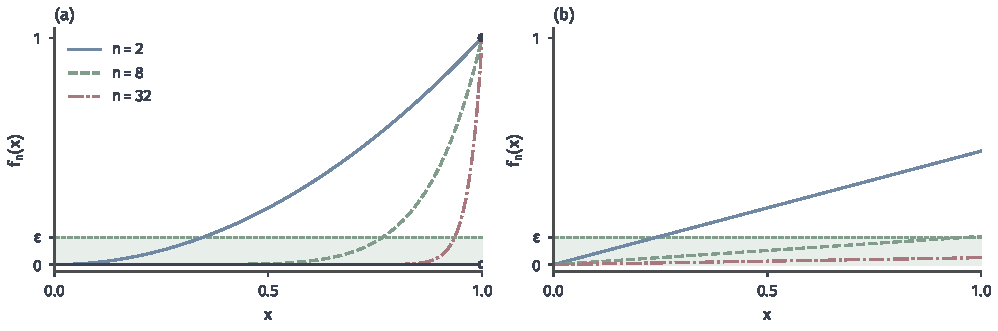
\includegraphics[width=169.0mm]{figures/01-mathematical-preliminaries-upper/01-mathematical-language-combinatorics-analysis-optimization/matplotlib/chapter3-concept-processes/pointwise-uniform-errors.pdf}
 \caption{(a) $f_n=x^n$在$[0,1]$上，黑点与空心点标记逐点极限$\mathbb I_{\{1\}}$；任意有限$n$仍有靠近$1$的输入使误差接近$1$。(b) $g_n=x/n$对所有输入误差均不超过$1/n$。两图绘$n=2,8,32$，绿色带为零附近的$0.12$误差范围；左图在$x=1$处的极限值是$1$，不能将此带误作对该点的误差要求。}
 \label{fig:analysis-process-pointwise-uniform-errors}
\end{figure*}

\paragraph{几乎处处收敛不保证点态收敛}
在$[0,1]$上令$f_n(x)=n\mathbb I_{\{0\}}(x)$，并指定极限为零函数。
在每个$x\neq0$处函数列恒为零，因此几乎处处趋零；在$x=0$处却趋于无穷，连有限的点态极限都不存在。
每个$f_n$都与零函数几乎处处相等，若将原点处的值全部改为零，所得另一列函数便一致收敛到零。
所以零测改值不影响勒贝格积分，却可能改变原来这列函数的点态收敛和一致收敛；这两种收敛检查的是实际取值，不能只由几乎处处等价类决定。

\subsubsection{极限与连续}

逐点收敛只说明固定输入处的变化，不能统一控制邻近输入之间的差，因此不自动保留连续性。
一致收敛提供共同的函数值误差，连续性便可传给极限；局部一致收敛也足够，因为检查某点连续只需它附近的输入。

\paragraph{连续函数的一致极限}
用连续函数逼近一个函数时，需要确认共同误差控制能否把连续性传给极限。
\begin{theorem}[一致极限保持连续性]
\label{thm:analysis-uniform-continuity-limit}
设$X\subseteq\mathbb R$，连续函数$f_n:X\to\mathbb R$一致收敛到$f$，则$f$在$X$上连续。
\end{theorem}
\begin{proof}
固定$a\in X$及$\varepsilon>0$，先选$N$使$\sup_X|f_N-f|<\varepsilon/3$，再由$f_N$在$a$处连续选$\delta$。当$x\in X$且$|x-a|<\delta$时，
\[
 |f(x)-f(a)|
 \leq |f(x)-f_N(x)|+|f_N(x)-f_N(a)|+|f_N(a)-f(a)|<\varepsilon.
\]
所以$f$连续。这里先固定一个对所有输入都适用的$N$，再调用单个$f_N$的连续性。
\end{proof}

前面幂函数列的反例已给出不连续的点态极限，所以逐点收敛不能代替一致收敛。还需区分另一个逆向问题：若将同一函数列限制到$[0,1)$，点态极限为连续函数$0$，但$\sup_{[0,1)}x^n=1$，仍不一致趋零。因此极限连续也不能反推一致收敛。


局部一致收敛指每个点都有一个相对邻域，使函数列在该邻域上一致收敛；将同一定理限制到该邻域，即得极限在该点连续。

同样的三项误差估计也适用于度量空间上的连续函数列，而不只是一元实函数；它保留连续性所用的是共同误差尺度，几乎处处收敛的零测例外不能提供这一尺度。

\subsubsection{极限与微分}

求导要比较缩小输入尺度后的差商，因此函数值一致接近仍可能漏掉快速振荡或尖点。
一种足够的控制是导数一致收敛并固定一个函数值；若只控制导数的积分误差，则可得到绝对连续及几乎处处导数的结论，结论强度不同。

\paragraph{一致收敛与导数}
函数值的一致收敛不能保证导数收敛。例如$f_n(x)=\sin(nx)/n$在$[0,2\pi]$上一致趋于零，因为$\sup|f_n|\leq1/n$；导数$f_n'(x)=\cos(nx)$在$x=0$处始终为$1$，连逐点趋零都不成立。

一致极限还可能不可导。令$f_\varepsilon(x)=\sqrt{x^2+\varepsilon^2}$，则
\[
 0\leq f_\varepsilon(x)-|x|
 =\frac{\varepsilon^2}{\sqrt{x^2+\varepsilon^2}+|x|}\leq\varepsilon.
\]
所以它们在实轴上一致趋于$|x|$，但极限在原点不可导。各近似函数的导数为$x/\sqrt{x^2+\varepsilon^2}$；对$x\neq0$趋于$\operatorname{sign}(x)$，其中正数的符号为$1$、负数的符号为$-1$，在原点导数恒为零。即使规定$\operatorname{sign}(0)=0$，这种导数收敛也不一致：取$x_\varepsilon=\varepsilon^2$，导数值趋零，而$\operatorname{sign}(x_\varepsilon)=1$，误差趋于一。

\paragraph{连续可微函数列导数的一致收敛}
若控制的是导数，还需固定一个函数值，才能排除任意竖直平移。
\begin{theorem}[一致导数逼近与求导保持]
\label{thm:analysis-uniform-derivative-limit}
设$a<b$，$f_n\in C^1([a,b])$。若某个$x_0\in[a,b]$满足$f_n(x_0)\to c$，且$f_n'$在$[a,b]$上一致收敛到$g$，则$f_n$一致收敛到某个$f\in C^1([a,b])$，并有$f(x_0)=c$、$f'=g$。
\end{theorem}
\begin{proof}
对$f_n-f_m$使用中值定理，得到
\[
 |f_n(x)-f_m(x)|\leq |f_n(x_0)-f_m(x_0)|+(b-a)\lVert f_n'-f_m'\rVert_\infty.
\]
右侧随$m,n\to\infty$一致趋零，所以$f_n$一致柯西。实值函数列的一致柯西判据给出一致极限$f$，且$f(x_0)=c$。$f,g$均为连续函数的一致极限，因而连续。

还须证明$f'=g$。给定$\varepsilon>0$，取$N$使$n\geq N$时$\lVert f_n'-g\rVert_\infty<\varepsilon$。对$n,m\geq N$及$x\neq y$，中值定理给出
\[
 |(f_n-f_m)(y)-(f_n-f_m)(x)|\leq2\varepsilon|y-x|.
\]
固定$n\geq N$，令$m\to\infty$，再除以$|y-x|$，可知$f$与$f_n$的差商相差至多$2\varepsilon$。因此
\[
 \begin{aligned}
 \left|\frac{f(y)-f(x)}{y-x}-g(x)\right|
 &\leq2\varepsilon+
 \left|\frac{f_n(y)-f_n(x)}{y-x}-f_n'(x)\right|\\
 &\quad+|f_n'(x)-g(x)|.
 \end{aligned}
\]
先固定这个$n$再令$y\to x$，中间一项趋零，最后一项小于$\varepsilon$。由$\varepsilon$任意，得到$f'(x)=g(x)$；端点使用单侧差商。
\end{proof}
若没有单点收敛条件，$f_n(x)=n$的导数虽全为零，函数值却不收敛；若只有函数值一致收敛，上面的振荡和平滑绝对值例子已经说明求导可能失败。这个证明只用中值定理与一致柯西条件；它不要求先把函数值写成导数的积分。

\paragraph{绝对连续函数列导数按积分误差的收敛}
导数未必一致收敛，但若其绝对误差的总累计趋零，仍能控制所有端点的函数增量。
下面用勒贝格积分给出这一条件，结论不额外承诺极限导数连续。
\begin{theorem}[导数积分误差控制的极限]
\label{thm:analysis-integral-derivative-limit}
设$f_n$在$[a,b]$上绝对连续，$g$勒贝格可积，且某个$x_0\in[a,b]$满足$f_n(x_0)\to c$。
若
\[
 \int_a^b|f_n'(t)-g(t)|\,\mathrm dt\longrightarrow0,
\]
则$f_n$一致收敛到绝对连续函数$f(x)=c+\int_{x_0}^xg(t)\,\mathrm dt$，且$f'=g$几乎处处。
\end{theorem}
\begin{proof}
绝对连续函数的基本定理给出$f_n(x)=f_n(x_0)+\int_{x_0}^xf_n'(t)\,\mathrm dt$，因而
\[
 \sup_{x\in[a,b]}|f_n(x)-f(x)|
 \leq|f_n(x_0)-c|+\int_a^b|f_n'-g|\,\mathrm dt\longrightarrow0.
\]
可积函数的累计绝对连续，且导数几乎处处等于$g$，故得结论。
\end{proof}
导数一致收敛定理给出$C^1$极限；这里的积分误差条件只保证绝对连续和几乎处处求导。

\subsubsection{极限与积分}

积分要控制的是整个范围的累计，逐点误差变小未必排除越来越窄的高峰，也未必排除向更远处扩散的贡献。
先检查极限是否可测，再比较四种条件：有限测度上的一致收敛、非负单调收敛、仅非负时的单向估计，以及共同可积上界下的积分交换。

\paragraph{可测函数的逐点极限}
收敛定理还要对极限函数积分，因此必须先确认极限仍是可测函数。
可数个可测函数的上确界、下确界可测，例如$\{\sup_nf_n>a\}=\bigcup_n\{f_n>a\}$。因此
\[
 \liminf_nf_n=\sup_N\inf_{n\geq N}f_n,\qquad
 \limsup_nf_n=\inf_N\sup_{n\geq N}f_n
\]
都可测；逐点极限存在时也可测。连续函数的逐点极限可能不连续，而可测函数的这一封闭性，使函数逼近更容易留在同一类对象中。

\paragraph{逐点收敛的反例}
每个输入处的误差趋零，未必排除面积集中的窄峰；下面固定峰的形状，比较降低总面积与保持总面积两种变化。
用同一形状比较两列连续函数。在$[0,1]$上记$t_+=\max\{t,0\}$，令
\begin{equation}
 b_n(x)=(1-|2nx-1|)_+,\qquad a_n(x)=2n\,b_n(x),\qquad n\geq1.
\label{eq:measurable-continuous-spikes}
\end{equation}
它们只可能在$[0,1/n]$上非零，顶点位于$1/(2n)$，高度分别为$1$和$2n$。
固定$x>0$后，充分大的$n$使$x>1/n$；在$x=0$处两列始终为零，所以都处处趋零。
由三角形面积计算，它们的勒贝格积分满足
\[
 \int_0^1b_n\,\mathrm dx=\frac1{2n},\qquad \int_0^1a_n\,\mathrm dx=1.
\]
两列均不一致趋零，因为最大高度没有趋零。第一列的积分仍趋零；第二列却有
\begin{equation}
 \int_0^1a_n(x)\,\mathrm dx=1,
 \qquad \int_0^1\lim_{n\to\infty}a_n(x)\,\mathrm dx=0.
\label{eq:analysis-continuous-spike-integral-failure}
\end{equation}
这里各项及极限都可积：一致收敛是保证交换的充分条件，逐点收敛却不足够。
峰顶随$n$移动，逐点极限最终看不到它，积分仍保留整个面积；
下面将检查共同可积上界能否控制这项集中贡献。

\paragraph{有限测度上一致收敛下的积分极限}
\label{sec:analysis-classical-limit-integral}
一致误差乘总测度给出积分误差，因此它在有限测度范围上足以交换极限与积分。
这需要总测度有限，也需要各项确实可积。
\begin{theorem}[有限测度上的一致收敛与积分]
\label{thm:analysis-uniform-lebesgue-integral-limit}
设$(X,\mathcal A,\mu)$为测度空间，$\mu(X)<\infty$，实值可测函数$f_n$可积，并在$X$上一致收敛到$f$。
则$f$可积，且
\begin{equation}
 \int_X|f_n-f|\,\mathrm d\mu
 \leq\mu(X)\|f_n-f\|_\infty\longrightarrow0,
 \qquad \int_Xf_n\,\mathrm d\mu\longrightarrow\int_Xf\,\mathrm d\mu.
\label{eq:analysis-uniform-riemann-limit}
\end{equation}
\end{theorem}
\begin{proof}
逐点极限$f$可测。一致收敛保证可选一个$n_0$使$\|f-f_{n_0}\|_\infty<1$，因此
$\int|f|\leq\int|f_{n_0}|+\mu(X)<\infty$。
对充分大的$n$，把有限的共同误差积分，得到所述绝对误差界；积分差的绝对值不超过这项误差积分。
\end{proof}
在无限测度范围上，一致收敛也不足：$f_n=n^{-1}\mathbb I_{[0,n]}$在实轴上一致趋零，积分却恒为$1$。
因此，下列三项测度论结论改用单调性或共同可积上界控制总累计。

\paragraph{非负可测函数列的单调递增收敛}
记$f_n(x)\uparrow f(x)$表示每个固定$x$处的数列单调增加且趋于$f(x)$；允许忽略零测例外时，例外须包含在同一个可测零测集中。简单函数从下方逼近非负函数时正是这样逐步增加的，下面把阶梯逼近中的积分极限关系推广到任意递增的非负可测函数列\scite{math-folland1999real}。
\begin{theorem}[单调收敛定理]
\label{thm:analysis-monotone-convergence}
设$f_n,f:X\to[0,\infty]$可测，且$f_n(x)\uparrow f(x)$几乎处处，则它们的勒贝格积分满足
\[   \lim_{n\to\infty}\int_X f_n\,\mathrm{d}\mu   =   \int_X f\,\mathrm{d}\mu. \]
两边都允许取$+\infty$。
\end{theorem}
\begin{proof}
把单调性或收敛关系失效的可测零测集并为$N$，并将$f_n$与$f$在$N$上都改为$0$。
修改后的函数仍可测且积分不变，所以可假定$f_n\uparrow f$逐点成立。由
$0\leq f_n\leq f$，积分序列单调不减且
\[   L:=\lim_{n\to\infty}\int f_n\,\mathrm{d}\mu   \leq\int f\,\mathrm{d}\mu. \]
还需证明反向不等式。任取满足$0\leq s\leq f$的简单函数，将它写为 $s=\sum_{j=1}^m a_j\mathbb{I}_{E_j}$，其中$a_j>0$且$E_j$两两不交。固定 $c\in(0,1)$，定义
\[   E_{j,n}   =   E_j\cap\{x:f_n(x)\geq ca_j\}. \]
由于$f_n\uparrow f$且$f\geq a_j$于$E_j$，有$E_{j,n}\uparrow E_j$。
第~\ref{sec:analysis-set-measure-continuity}节已由可数可加性证明测度对递增集合连续，
故$\mu(E_{j,n})\uparrow\mu(E_j)$。同时
\[   f_n   \geq   c\sum_{j=1}^m a_j\mathbb{I}_{E_{j,n}}, \]
从而
\[   L   \geq   \lim_{n\to\infty}   c\sum_{j=1}^m a_j\mu(E_{j,n})   =   c\int s\,\mathrm{d}\mu. \]
先令$c\uparrow1$，再对所有$0\leq s\leq f$的简单函数取上确界。根据非负积分的定义~\eqref{eq:analysis-nonnegative-lebesgue-integral}， $L\geq\int f\,\mathrm{d}\mu$。与前一不等式合并即得结论。
\end{proof}

非负性避免正负无穷相消，单调性保证已经积累的质量不会在后续消失。定理不要求存在可积的统一上界，也不要求各$\int f_n$有限。


在$[0,1]$上枚举有理数为$q_1,q_2,\ldots$，令$E_n=\{q_1,\ldots,q_n\}$。
$\mathbb I_{E_n}$递增到$\mathbb I_{\mathbb Q\cap[0,1]}$，各项及极限的勒贝格积分都为零，单调收敛保证这一逼近不离开可测积分框架。
但非负递增不保证有限积分：在$(0,\infty)$上，$\mathbb I_{(0,n)}\uparrow1$，积分从$n$增加到无穷，仍符合单调收敛等式。

\paragraph{非负可测函数列的下极限与积分估计}

若删除单调要求，只保留非负性，连续尖峰$a_n$说明积分等式可能失败，但仍有一个方向的界。对可能不收敛的函数列，可以用每个位置的下极限比较尾部贡献。

\begin{lemma}[Fatou引理]
\label{lem:analysis-fatou}
若$f_n:X\to[0,\infty]$可测，则关于$\mu$的勒贝格积分满足
\begin{equation}
  \int_X\liminf_{n\to\infty}f_n\,\mathrm{d}\mu
  \leq
  \liminf_{n\to\infty}\int_Xf_n\,\mathrm{d}\mu.
\label{eq:analysis-fatou}
\end{equation}
\end{lemma}
\begin{proof}
令$g_n=\inf_{k\geq n}f_k$。则$g_n$可测， $0\leq g_n\uparrow\liminf_k f_k$。由单调收敛定理，
\[   \int\liminf_k f_k\,\mathrm{d}\mu   =   \lim_{n\to\infty}\int g_n\,\mathrm{d}\mu. \]
对每个$k\geq n$都有$g_n\leq f_k$，故
\[   \int g_n\,\mathrm{d}\mu   \leq   \inf_{k\geq n}\int f_k\,\mathrm{d}\mu. \]
令$n\to\infty$便得到式~\eqref{eq:analysis-fatou}。
\end{proof}

非负条件也不能直接删除。令$g_n=n\mathbb I_{(0,1/n)}$，它是集中在短区间上的矩形尖峰，处处趋零且积分恒为$1$。若改取$u_n=-g_n$，则
$\liminf_n u_n=0$处处成立，而$\int u_n=-1$；原不等式会变成错误的$0\leq-1$。
若另有共同的可积下界$h$使$u_n\geq h$，则可以对$u_n-h\geq0$应用Fatou，
再移去有限的$\int h$。可积下界是可用的推广条件，不是无条件允许负值。

Fatou通常只给一个方向。对式~\eqref{eq:measurable-continuous-spikes}中的$a_n$，左边为零、右边为一，不等式严格成立。积分贡献集中在越来越小的区间内，逐点极限没有保留它。下面图~\ref{fig:analysis-convergence-obstacles}左侧的矩形尖峰提供同样的机制：它与连续三角尖峰的连续性不同，积分失效的原因相同。右侧回顾前面的求导反例，说明积分与导数需要各自的误差控制。

\paragraph{共同可积上界下的收敛与积分}

若函数会振荡或有正负值，单调条件未必可用，可以改用同一个非负可积函数$g$控制所有$|f_n|$，让局部高峰和远处尾部都受有限总量限制。每个$f_n$分别可积还不够，下面要求的是一项覆盖整列函数的共同控制。

\begin{theorem}[支配收敛定理]
\label{thm:analysis-dominated-convergence}
设$f_n,f:X\to\mathbb{R}$可测，$f_n\to f$几乎处处，并且存在非负勒贝格可积函数$g$使
$|f_n|\leq g$几乎处处对所有$n$成立，则$f$勒贝格可积，而且勒贝格积分满足
\[   \lim_{n\to\infty}\int_Xf_n\,\mathrm{d}\mu   =   \int_Xf\,\mathrm{d}\mu. \]
此外，$\int|f_n-f|\,\mathrm{d}\mu\to0$。
\end{theorem}
\begin{proof}
把收敛或控制条件失效的可测零测集的可数并记为$N$，并将$f_n,f,g$在$N$上都改为
$0$。这些函数仍可测且积分不变，因而下述关系可以按逐点意义使用。
由$|f_n|\leq g$并取逐点极限可得$|f|\leq g$几乎处处，所以$f$可积。函数$g+f_n$与$g-f_n$均非负。对它们分别使用Fatou引理，
\begin{align*}
  \int g+\int f
  &\leq
  \int g+\liminf_{n\to\infty}\int f_n,\\
  \int g-\int f
  &\leq
  \int g-\limsup_{n\to\infty}\int f_n.
\end{align*}
由于$\int g<\infty$，可以从两边减去它，得到
\[   \int f   \leq\liminf_n\int f_n   \leq\limsup_n\int f_n   \leq\int f. \]
故积分收敛到$\int f$。

最后，$|f_n-f|\to0$几乎处处，且 $|f_n-f|\leq2g$。再对非负函数$|f_n-f|$应用刚证明的积分交换结论，得到 $\int|f_n-f|\,\mathrm{d}\mu\to0$。
\end{proof}


在$[0,1]$上，幂函数列$x^n$几乎处处趋零，且被可积常数一支配，故积分趋零；这与它不一致收敛没有矛盾。连续尖峰$b_n$也满足$0\leq b_n\leq1$，所以支配收敛给出$\int b_n\to0$。面积保持为一的$a_n$则没有共同可积支配，下面直接检查这一缺口。

假设存在非负可积的$g$使$g\geq a_n$几乎处处对每个$n$成立。
则$1=\int_0^1a_n\leq\int_{[0,1/n]}g$。
但$[0,1/n]$的测度趋零，前面证明的绝对积分的小集合估计使右侧趋零，矛盾。
所以这里并非支配函数暂时没有找到，而是这种可积支配根本不存在。

贡献也可以向无穷远移动：在$\mathbb R$上令$f_n=\mathbb I_{[n,n+1)}$，则处处趋零且积分恒为一。它虽共用常数上界一，那个上界在整条实轴上不可积。支配函数本身可以无界；后面的反常积分部分计算端点附近的累计后，再给出这样的例子。

\begin{figure*}[htbp]
  \centering
  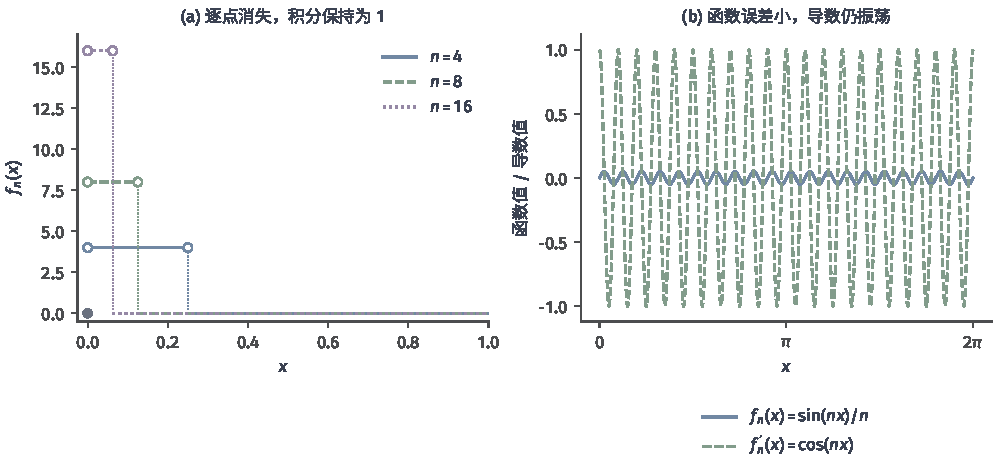
\includegraphics[width=169.0mm]{figures/01-mathematical-preliminaries-upper/01-mathematical-language-combinatorics-analysis-optimization/matplotlib/analysis-convergence-obstacles/figure.pdf}
  \caption{两种交换运算的障碍。左图的尖峰支撑不断收缩，但高度同步增长，每条曲线的积分仍为$1$；开圆点标出不取的上端点，竖虚线仅提示跳跃。右图取$n=20$，$\sin(nx)/n$的函数幅度很小，导数$\cos(nx)$仍有单位幅度。两图均为按给定函数公式构造的教学示例。}
 \label{fig:analysis-convergence-obstacles}
\end{figure*}

表~\ref{tab:analysis-interchange-conditions}汇总极限与勒贝格积分交换的不同条件。积分等式成立的依据来自这些条件，不能仅由已经存在的点态极限推出。
\begin{table*}[htbp]
 \centering\small
 \begin{tabularx}{\linewidth}{@{}lXX@{}}
 \toprule
 结果 & 核对的条件 & 可得到的结论\\
 \midrule
 有限测度上一致收敛 & 各项可积，且全部输入的误差一致趋零 & 极限可积，积分可交换极限\\
 单调收敛 & 非负可测函数逐点或几乎处处递增 & 极限与积分相等，允许无穷值\\
 Fatou引理 & 非负可测函数列 & 先取下极限再积分，不超过先积分再取下极限的结果\\
 支配收敛 & 几乎处处收敛，且共用一个可积绝对上界 & 积分可交换极限，并有$\int|f_n-f|\,\mathrm d\mu\to0$\\
 \bottomrule
 \end{tabularx}
 \caption{极限与勒贝格积分之间的交换条件。表中的测度、可测性和统一控制属于结论的假设。}
 \label{tab:analysis-interchange-conditions}
\end{table*}


这些结论控制的运算不同：保留连续性使用共同函数值误差，交换微分还要控制导数；交换积分则检查有限测度、非负单调性或共同可积支配等相应条件。表~\ref{tab:analysis-interchange-conditions}中的条件及前面的反例给出了各自的适用边界。

\subsection{函数项级数的极限}
\label{sec:analysis-function-series-limits}

函数列的极限比较一列已经给定的函数；函数项级数则把不断加入的函数项累计起来。
给定$u_n:X\to\mathbb R$，记部分和$S_N(x)=\sum_{n=1}^Nu_n(x)$，研究$\sum_{n=1}^\infty u_n(x)$就是研究函数列$(S_N)$。
下面先按部分和区分收敛方式，再判断何时收敛，以及求导或积分能否移入无穷求和。

\subsubsection{收敛方式与判别}

部分和把级数化成函数列，前面几种收敛方式都可以沿用，但必须说明它们约束的是部分和，而不是单个函数项$u_n$。

\paragraph{点态收敛}
若对每个$x\in X$，实数级数$\sum_nu_n(x)$有有限和$u(x)$，就称函数项级数点态收敛到和函数$u$，即$S_N(x)\to u(x)$。
尾部起点可以随$x$改变。特别地，$u_n(x)\to0$只是必要条件，不能代替部分和收敛。

\paragraph{点态收敛的判据}
未知和函数时，比较两个较晚的部分和；它们的差是一段有限尾和，因此点态收敛等价于：
\[
 \begin{gathered}
 \forall x\in X,\quad\forall\varepsilon>0,\quad\exists N=N(x,\varepsilon),\\
 m>n\geq N\Longrightarrow
 \left|\sum_{k=n+1}^{m}u_k(x)\right|<\varepsilon.
 \end{gathered}
\]
这是将定理~\ref{thm:analysis-pointwise-cauchy-criterion}用于$S_N$，与数项级数逐点使用柯西准则完全一致。

\paragraph{一致收敛}
若部分和函数列在$X$上一致收敛到$u$，就称函数项级数在$X$上一致收敛，即
\[
 \sup_{x\in X}|S_N(x)-u(x)|\longrightarrow0.
\]
同一个$N$控制全部输入处的剩余和。例如在$[0,1)$上，$\sum_{n=0}^\infty x^n$逐点收敛到$1/(1-x)$，但每个有限部分和有界而和函数无界，不可能一致收敛。
若每个$u_n$连续，有限部分和也连续，一致收敛便由定理~\ref{thm:analysis-uniform-continuity-limit}保证和函数连续。

\paragraph{一致收敛的判据}
若希望得到一致收敛，就要把尾部起点放在选择输入之前。
由定理~\ref{thm:analysis-uniform-cauchy-criterion}，一致收敛当且仅当
\[
 \begin{gathered}
 \forall\varepsilon>0,\quad\exists N,\quad\forall x\in X,\\
 m>n\geq N\Longrightarrow
 \left|\sum_{k=n+1}^{m}u_k(x)\right|<\varepsilon.
 \end{gathered}
\]
这里不预先指定和函数，实数的完备性先提供各点极限，共同尾和界再使收敛一致。

\paragraph{几乎处处收敛}
在测度空间$(X,\mathcal A,\mu)$上，若存在一个可测零测集$E$，使$S_N(x)$在每个$x\notin E$处收敛到$u(x)$，就称级数几乎处处收敛。
各函数项可测时，可以把和函数在$E$上取零以保留可测性。它与点态收敛的区别是允许固定的零测例外，并未提供全域共同的误差界。

\paragraph{绝对收敛}
若对每个$x$都有$\sum_n|u_n(x)|<\infty$，就称函数项级数在各点绝对收敛；只在零测集外成立时称几乎处处绝对收敛。
这能保证相应位置的级数收敛，却不自动给出一致收敛；后者还需要全部输入共同适用的尾和控制。

\paragraph{Weierstrass判别法}
逐一估计所有输入处的尾和可能困难。若每项都能用一个与输入无关的非负数控制，就可把函数项级数归约为已知的数项级数。
\begin{theorem}[Weierstrass判别法]
\label{thm:analysis-weierstrass-series-test}
设$X$非空，$u_n:X\to\mathbb R$。若存在非负实数$M_n$使
\[
 \forall x\in X,\quad |u_n(x)|\leq M_n,
 \qquad \sum_{n=1}^{\infty}M_n<\infty,
\]
则$\sum_nu_n$在每个$x$处绝对收敛，并在$X$上一致收敛到某个实值函数$u$。
此外，截断误差满足
\[
 \sup_{x\in X}\left|u(x)-\sum_{n=1}^Nu_n(x)\right|
 \leq\sum_{n>N}M_n\longrightarrow0.
\]
\end{theorem}
\begin{proof}
对每个固定$x$，比较判别给出$\sum_n|u_n(x)|\leq\sum_nM_n<\infty$，故和$u(x)$存在。
对任意$m>N$，三角不等式给出$|\sum_{n=N+1}^m u_n(x)|\leq\sum_{n>N}M_n$。
令$m\to\infty$并对$x$取上确界，就得到所述误差界；数项级数的尾和趋零，故收敛一致。
\end{proof}
例如在$[-1,1]$上，$u_n(x)=x^n/2^n$满足$|u_n(x)|\leq2^{-n}$，而$\sum_{n>N}2^{-n}=2^{-N}$。
这个共同的几何尾和控制全部输入处的截断误差；每个函数项连续，所以和函数也连续。
判别法是充分条件，不能把“没有找到这样的$M_n$”当成不一致收敛的证明。

\subsubsection{逐项求导}

部分和总可以有限次求导，问题在于求导后再取极限，是否得到和函数的导数。
单靠原级数一致收敛仍不够；下面把控制施加在导数级数，并用一个点的函数值确定累计常数。
\begin{theorem}[函数项级数的逐项求导]
\label{thm:analysis-function-series-differentiation}
设$u_n\in C^1([a,b])$。若存在$x_0\in[a,b]$使$\sum_nu_n(x_0)$收敛，且导数级数$\sum_nu_n'$在$[a,b]$上一致收敛，则$\sum_nu_n$在$[a,b]$上一致收敛到某个$u\in C^1([a,b])$，且
\[
 u'(x)=\sum_{n=1}^{\infty}u_n'(x).
\]
\end{theorem}
\begin{proof}
取$S_N=\sum_{n=1}^Nu_n$，则$S_N(x_0)$收敛，$S_N'=\sum_{n=1}^Nu_n'$一致收敛。
将函数列导数的一致收敛结论（定理~\ref{thm:analysis-uniform-derivative-limit}）用于$S_N$，即得原级数一致收敛、和函数连续可微以及导数公式。
\end{proof}
例如可用Weierstrass判别法检查导数级数的一致收敛；这与直接检查原级数的共同上界是两件事。
若函数项只有绝对连续性，也可将定理~\ref{thm:analysis-integral-derivative-limit}用于部分和：单点级数收敛且导数部分和按绝对误差积分趋于某个可积函数$g$时，和函数绝对连续，并有$u'=g$几乎处处。
这里$g$是导数部分和的积分误差极限，不能额外断言导数级数在每个点都收敛。

\subsubsection{逐项积分}

将有限部分和的积分写成有限和总是允许的，能否再令项数趋于无穷，则取决于部分和的积分控制。
非负项、绝对积分总和有限以及有限测度上的一致收敛，给出三种不同的充分条件。

\paragraph{非负函数项级数的逐项积分}
非负项使部分和递增，因此可以直接使用前面的单调收敛结论，不要求总积分有限。
\begin{theorem}[非负函数项级数的逐项积分]
\label{thm:analysis-nonnegative-series-integration}
若$u_n:X\to[0,\infty]$可测，则
\[
 \int_X\sum_{n=1}^{\infty}u_n\,\mathrm d\mu
 =\sum_{n=1}^{\infty}\int_Xu_n\,\mathrm d\mu,
\]
两边均允许为$+\infty$。
\end{theorem}
\begin{proof}
非负部分和$S_N$递增到$\sum_nu_n$。用单调收敛定理交换极限与积分，再对每个$S_N$用有限加法，即得等式。
\end{proof}

\paragraph{绝对积分总和有限时的逐项积分}
有正负项时，绝对累计可以同时控制无限求和中的抵消及积分误差。
下面的条件既保证和函数可积，也保证部分和按绝对误差积分趋于和函数。
\begin{theorem}[绝对积分可求和的函数项级数]
\label{thm:analysis-absolutely-integrable-series}
若$u_n:X\to\mathbb R$可测且$\sum_n\int_X|u_n|\,\mathrm d\mu<\infty$，则$\sum_nu_n$几乎处处绝对收敛。
将和函数在绝对值级数发散的可测零测集上定义为零，所得$u$可积，并有
\[
 \int_X\left|u-\sum_{n=1}^Nu_n\right|\,\mathrm d\mu
 \leq\sum_{n>N}\int_X|u_n|\,\mathrm d\mu\longrightarrow0,
\]
从而
\[
 \int_Xu\,\mathrm d\mu=\sum_{n=1}^{\infty}\int_Xu_n\,\mathrm d\mu.
\]
\end{theorem}
\begin{proof}
由非负级数的逐项积分，$G=\sum_n|u_n|$满足$\int_XG\,\mathrm d\mu<\infty$，故$G<\infty$几乎处处。
在可测零测集$E=\{G=\infty\}$之外，级数绝对收敛，且$|u|\leq G$；在$E$上取$u=0$后，$u$仍可测且可积。
对几乎每个$x$，$|u(x)-S_N(x)|\leq\sum_{n>N}|u_n(x)|$。
对这一不等式积分，再对右侧非负尾级数逐项积分，得到所述误差界。
积分差不超过绝对误差积分，而有限部分和满足$\int S_N=\sum_{n=1}^N\int u_n$，令$N\to\infty$便得到结论。
\end{proof}

\paragraph{有限测度上一致收敛时的逐项积分}
还有一种充分条件直接约束部分和的共同误差，而不要求绝对积分的总和有限。
若$\mu(X)<\infty$、各$u_n$可积，且部分和$S_N$一致收敛到$u$，则定理~\ref{thm:analysis-uniform-lebesgue-integral-limit}给出
\[
 \int_Xu\,\mathrm d\mu
 =\lim_{N\to\infty}\int_XS_N\,\mathrm d\mu
 =\sum_{n=1}^{\infty}\int_Xu_n\,\mathrm d\mu.
\]
这里的关键是有限总测度乘一致误差趋零；它与上一段的绝对可求和条件应分别检查。

\subsection{反常积分}
\label{sec:analysis-improper-integrals}

前面的有限区间计算还留下两个问题：积分范围延伸到无穷远时怎样累计，函数在端点或内部位置无界时怎样累计。
这两类问题通常称为\term{反常积分}（improper integral）。下面先分别说明定义与截断方式，再集中判断何时可积。
本节沿用勒贝格积分约定：非负函数的积分允许为无穷，有符号函数的有限可积性要求绝对值积分有限；截断用来计算已有的积分，不把指定顺序下的抵消另算作有限勒贝格积分。

\subsubsection{无穷区间上反常积分的定义}

先设$f$在每个有限区间$[a,R]$上勒贝格可积，唯一待处理的部分是无穷远处的尾部。
把积分范围延伸到半轴，就得到这一类反常积分的记号。
\begin{definition}[无穷区间上的反常积分]
\label{def:analysis-improper-infinite-interval}
设$f:[a,\infty)\to\mathbb R$可测，且在每个$[a,R]$上可积。
将$[a,\infty)$上的勒贝格积分记为
\[
 \int_a^\infty f(x)\,\mathrm dx:=\int_{[a,\infty)}f\,\mathrm dm,
\]
称为无穷区间上的反常积分。
若$f\geq0$，该值属于$[0,\infty]$；若$f$有正负值，本节讨论其有限积分时要求$\int_a^\infty|f|<\infty$。
\end{definition}
这个记号可以通过有限范围上的计算求值。非负时由单调收敛，有
\[
 \int_a^\infty f(x)\,\mathrm dx
 =\lim_{R\to\infty}\int_a^R f(x)\,\mathrm dx,
\]
允许为无穷；有符号且绝对可积时，对$f\mathbb I_{[a,R]}$使用$|f|$支配，也得到同一有限等式。
严格说，可先沿$R_n\uparrow\infty$应用函数列的收敛结论；非负累计的单调性或遗漏范围的绝对积分趋零，再保证任意$R\to\infty$时结论相同。

左半轴作相同处理。整个实轴上还需分别处理左右两端：对任意固定$c\in\mathbb R$，$f$可积当且仅当两侧的绝对值积分都有限，此时
\[
 \int_{\mathbb R}f\,\mathrm dm
 =\int_{(-\infty,c]}f\,\mathrm dm+\int_{(c,\infty)}f\,\mathrm dm.
\]
只知道对称截断$[-R,R]$中的正负抵消稳定，不能代替左右两侧可积。

\subsubsection{无界函数反常积分的定义}

范围有限时，函数仍可能在端点附近无界。先避开该端点计算，再检查遗漏的短区间是否保留了不可忽略的累计。
\begin{definition}[无界函数的反常积分]
\label{def:analysis-improper-unbounded-function}
设$f:(a,b]\to\mathbb R$可测，在每个$[c,b]$（$a<c<b$）上可积，并允许在$a$附近无界。
将$(a,b]$上的勒贝格积分记为
\[
 \int_a^bf(x)\,\mathrm dx:=\int_{(a,b]}f\,\mathrm dm,
\]
称为在端点$a$处的反常积分。
若$f\geq0$，该值允许为$+\infty$；若$f$有正负值，本节讨论其有限积分时要求$\int_{(a,b]}|f|\,\mathrm dm<\infty$。
\end{definition}
非负时，$f\mathbb I_{[c,b]}$随$c\downarrow a$逐步增加到$f$；有符号且绝对可积时，这些截断函数由$|f|$支配。
因此分别用单调收敛或支配收敛得到
\[
 \int_{(a,b]}f\,\mathrm dm=\lim_{c\downarrow a}\int_c^bf(x)\,\mathrm dx.
\]
若无界位置在右端点，就从左侧截断；若在内部点$s$，则把$(a,s)$与$(s,b)$分开累计，有符号有限积分要求两侧均绝对可积。
在单点上赋予可测有限值不改变勒贝格积分，因而判断可积性的是附近的累计，并非该点取了什么值。


图~\ref{fig:analysis-process-improper-two-truncations}对照两种截断：向外扩大累计范围，或从奇点附近逐渐补回遗漏范围。
\begin{figure*}[!htbp]
 \centering
 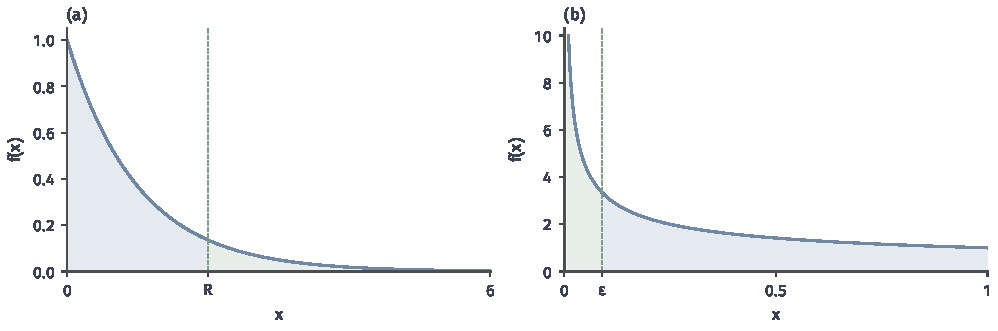
\includegraphics[width=169.0mm]{figures/01-mathematical-preliminaries-upper/01-mathematical-language-combinatorics-analysis-optimization/matplotlib/chapter3-concept-processes/improper-two-truncations.pdf}
 \caption{(a) $e^{-x}$在$[0,\infty)$上，以$R=2$截断，蓝区已计入，绿区属于遗漏尾部，其完整积分为$e^{-2}$；图只显示到$x=6$。(b) $x^{-1/2}$在$(0,1]$上，以$\varepsilon=0.09$截断，完整遗漏积分为$2\sqrt\varepsilon$。右图曲线只绘$x\geq0.01$，未画出的更近零点部分仍属积分范围。}
 \label{fig:analysis-process-improper-two-truncations}
\end{figure*}

\subsubsection{反常积分的可积性}

两种截断都可以写为递增可测范围$E_n\uparrow X$：范围不断延伸，或者从被避开的奇异位置逐步收回遗漏部分。
因此可以用同一个判据回答可积性问题，随后再用截断积分或原函数计算具体数值。

\paragraph{简单函数与截断函数的积分收敛}
对非负可测$f$，前面的规范简单函数$s_n$逐点递增到$f$，单调收敛定理现在补上$\int s_n\uparrow\int f$。若$f$绝对可积，截断$f_n=\max\{-n,\min\{f,n\}\}$满足$f_n\to f$且$|f_n|\leq|f|$，支配收敛给出$\int|f_n-f|\to0$。在实轴上再令截断范围$[-n,n]$扩大，所得$f\mathbb I_{[-n,n]}$也被$|f|$支配；这与前面的无穷范围截断相对应，说明有限范围上的计算可以逼近全域积分。

\paragraph{非负函数的可积性}
非负累计随截断范围扩大而增加，存在有限积分的关键是这些累计能否被同一个有限常数控制。
\begin{theorem}[非负截断累计的有界判据]
\label{thm:analysis-improper-nonnegative-criterion}
设$f:X\to[0,\infty]$可测，$E_n$为递增可测集且$\bigcup_nE_n=X$。则
\[
 \int_Xf\,\mathrm d\mu<\infty
 \quad\Longleftrightarrow\quad
 \sup_n\int_{E_n}f\,\mathrm d\mu<\infty,
\]
并有$\int_Xf\,\mathrm d\mu=\lim_n\int_{E_n}f\,\mathrm d\mu$。
\end{theorem}
\begin{proof}
因为$0\leq f\mathbb I_{E_n}\uparrow f$，单调收敛定理使全域积分等于截断积分序列的极限，也就是其上确界。
因此全域积分有限恰好等价于这些截断积分有共同有限上界。
\end{proof}
在无穷半轴上可取$E_n=[a,a+n]$，在奇异端点$a$附近可取$E_n=[a+(b-a)/(n+1),b]$。
只知道每一个截断积分分别有限不够，还要检验它们是否共同有界。

若$0\leq f\leq g$几乎处处且$\int g<\infty$，则$\int f<\infty$。
反之，若$0\leq g\leq f$且$\int g=\infty$，则$\int f=\infty$。
例如在$(0,1)$上，用单调截断与幂函数原函数计算，得到
\[
 \int_0^1x^{-1/2}\,\mathrm dx=\lim_{n\to\infty}2(1-n^{-1/2})=2,
 \qquad
 \int_0^1x^{-1}\,\mathrm dx=\lim_{n\to\infty}\log n=+\infty.
\]
在$[1,\infty)$上，$\int_1^\infty x^{-2}\,\mathrm dx=1$，而$\int_1^\infty x^{-1}\,\mathrm dx=+\infty$。
这几项计算始终使用同一勒贝格积分定义，极限等式由单调收敛保证。

以正函数$x^{-p}$说明位置的重要性。对$p>0$，在$[2^k,2^{k+1}]$上的累计满足
\[
 2^{-p}2^{k(1-p)}\leq\int_{2^k}^{2^{k+1}}x^{-p}\,\mathrm dx\leq2^{k(1-p)}.
\]
这是把函数在该段的最小值和最大值分别乘区间长度。$p>1$时上界随$k$几何衰减，有限几何和有共同上界，所以尾部积分收敛；$0<p\leq1$时各段至少贡献一个不趋零的正量，累计发散。$p\leq0$时$x^{-p}\geq1$于$x\geq1$，也发散。

同样比较靠近$0$的各段$[2^{-(k+1)},2^{-k}]$，在$p>0$时累计介于$2^{k(p-1)}/2$与$2^{p-1}2^{k(p-1)}$之间，故局部累计恰在$p<1$时有限；$p\leq0$时函数还能连续延拓到$0$，本来就可积。于是$\int_0^1x^{-p}\,\mathrm dx$恰在$p<1$时有限，$\int_1^\infty x^{-p}\,\mathrm dx$恰在$p>1$时有限。分段常数比较与几何级数给出可积性的阈值，原函数则能进一步计算有限截断的具体数值。

\paragraph{有符号函数的可积性}
正负值抵消可能使截断积分保持有限，但可积性要求正、负两部分各自具有有限累计。
因此应把上一段的非负判据用于$|f|$，而不是用于有正负抵消的$f$。
\begin{theorem}[绝对截断累计的可积性判据]
\label{thm:analysis-improper-signed-criterion}
设$f:X\to\mathbb R$可测，$E_n\uparrow X$为可测范围，则$f$可积当且仅当
\[
 \sup_n\int_{E_n}|f|\,\mathrm d\mu<\infty.
\]
可积时，每个截断积分有限，且
\[
 \left|\int_Xf\,\mathrm d\mu-\int_{E_n}f\,\mathrm d\mu\right|
 \leq\int_{X\setminus E_n}|f|\,\mathrm d\mu\longrightarrow0.
\]
所以任意这样的递增穷尽都得到同一个积分值。
\end{theorem}
\begin{proof}
将非负截断判据用于$|f|$，即得充要条件。可积时，区域可加性把积分差写成遗漏范围上的积分，再用绝对值界得到误差不等式。
函数$|f|\mathbb I_{X\setminus E_n}$逐点趋零且由可积的$|f|$支配，故其积分趋零。
\end{proof}
绝对值尾部既用于判断可积性，也控制有限计算的误差。

例如$p>1$时，按$[2^jR,2^{j+1}R]$分段比较得到
\[
 \int_R^\infty x^{-p}\,\mathrm dx
 \leq R^{1-p}\sum_{j=0}^\infty2^{j(1-p)}
 =\frac{R^{1-p}}{1-2^{1-p}}\longrightarrow0.
\]
非负积分的区域可数可加性保证分段求和合法，几何尾和给出显式误差界。

有了$x^{-1/2}$的可积性，就能核对无界支配的例子：在$(0,1)$上，$x^n/\sqrt x\to0$处处，
且$0\leq x^n/\sqrt x\leq x^{-1/2}$，因此支配收敛保证积分趋零。
截断后由原函数计算也得$\int_0^1x^{n-1/2}\,\mathrm dx=(n+1/2)^{-1}\to0$。
支配条件要求共同上界的绝对累计有限，不要求上界本身有界。

积分有限要求正负两部分都有限，不能从某一列截断积分有有限极限直接推出。
下面的例子只说明这种推断为什么失效，不把截断相消作为新的积分规则。

连续函数也可能出现截断相消。在$[1,\infty)$上，分部积分给出
\[
 \int_1^R\frac{\sin x}{x}\,\mathrm dx
 =\cos1-\frac{\cos R}{R}-\int_1^R\frac{\cos x}{x^2}\,\mathrm dx.
\]
端点项有极限，最后一项由$x^{-2}$控制而绝对收敛，所以截断积分存在有限极限。
但在每个$[k\pi+\pi/6,k\pi+5\pi/6]$（$k\geq1$）上，$|\sin x|\geq1/2$，
故该段的绝对积分至少为$1/(3(k+1))$。
调和级数发散使$\int_1^\infty|\sin x|/x\,\mathrm dx=+\infty$；
这个有限截断极限依赖正负抵消，不是本章所用的有限勒贝格积分。

在$(-1,1)$上取$f(x)=1/x$，原点赋值为零。
正负部分的积分都为无穷，所以$f$没有有符号勒贝格积分值；但对称截断满足
\[
 \lim_{\varepsilon\downarrow0}\left(
 \int_{-1}^{-\varepsilon}\frac{\mathrm dx}{x}
 +\int_{\varepsilon}^{1}\frac{\mathrm dx}{x}\right)=0.
\]
这个对称相消极限称为柯西主值。它没有使$\int|f|$变有限，也没有定义出本章采用的勒贝格积分。
后续计算仍只使用非负广义积分或绝对可积函数的有限积分。

\FloatBarrier
